%% ============================================================
%% QCCK-Model 中文总文档（摘要 + 六章 + 参考文献）
%% 编译：xelatex（ctex 需要 xelatex 或 lualatex），跑两遍出目录
%%       Overleaf 中请确认 Menu -> Compiler 选 XeLaTeX
%% 结构：各章正文分别放在 chapter0_abstract_zh / chapter1_intro_zh /
%%       chapter2_related_zh / chapter3_qcck_zh / chapter4_qcckm_zh /
%%       chapter5_qcckm_exp_zh / chapter6_conclusion_zh / references
%%       （均为纯正文文件），由本文件统一编译。
%% 编号：摘要与参考文献用 \section*（不编号），故引言=1、相关工作=2、
%%       QCCK=3、QCCK-M=4、实验=5、结论=6。
%% 图：第五章插图由 \ifchfivefigs 开关控制，当前 true（含插图版）。
%%     插图文件在 ch5/figs/ 下，共 6 张。
%% ============================================================
\documentclass[10pt,a4paper]{article}

\usepackage{ctex}
\usepackage{amsmath,amssymb}
\usepackage{geometry}
\geometry{margin=2.5cm}
\usepackage{graphicx}
\usepackage{float}
\usepackage{algorithm}
\usepackage{algorithmic}
\usepackage{xcolor}
\usepackage{longtable}
\usepackage{tikz}
\usetikzlibrary{arrows.meta,positioning,fit,backgrounds}

\newif\ifchfivefigs
\chfivefigstrue



\begin{document}




%% ============================================================
%% 摘要（中文版）
%% 结构：① 研究背景+问题引出 → ② 本文内容 QCCK → ③ QCCK 基础上提出 QCCK-M
%%       ④ 实验（Beijing 11% + 可解释性） → ⑤ 研究意义 for future
%% 纪律：缩写英文全称只在摘要首次出现时给出一次；
%%       QCCK-M 的英文全称是 QCCK-Model，不是 QCCK-Mamba。
%% 编译：xelatex（ctex）
%% ============================================================

\section*{摘要}

（第一句研究背景）
针对这一问题，本文提出一种量子跨变量耦合核（Quantum Cross-Variable Coupling Kernel，QCCK），利用频域对齐、量子编码与量子核三个环节显式构造变量之间的耦合关系。
在此基础上，本文进一步构建面向多变量时间序列预测的模型 QCCK-Model（QCCK-M），整合输入预处理、主干编码器的逐层更新、跨变量耦合融合与预测输出，把 QCCK 嵌入主干编码器层之间，使显式度量得到的耦合矩阵直接参与跨变量信息融合。
多组实验结果表明，QCCK-M 在多个公开数据集上优于现有方法，其中在 Beijing 数据集上 MSE 降低 11\%；同时，耦合矩阵以显式数值呈现变量间的耦合强度，使模型所依据的变量关系可以被直接读取。
上述结果表明，QCCK 为多变量时间序列预测中的跨变量耦合建模提供了一种可显式度量、可解释的途径，有望为量子核方法在时间序列任务中的应用提供新的思路。

%% ============================================================
%% 第一章 引言（中文版）
%% 结构：P1 研究背景+问题引出 → P2 用 Quantum Kernel 解决上述问题
%%       → P3 Our Work → P4 主要贡献（3 条）+ 本文结构
%% 编译：xelatex（ctex）
%% 说明：全文遵循"用英文逻辑写中文"，句句有主谓宾、句间逻辑显式。
%%       引用示例统一采用"xxxx年，某某等提出……，通过……，实现了……"的句式。
%% ============================================================

\section{引言}

时间序列预测是一类依据历史观测推断系统未来演化状态的建模任务，其核心目标是从数据中学习系统的动态规律，为后续的调度与控制提供提前判断的依据。
作为深度学习中的一个重要方向，它把深度神经网络与时序分析相融合，形成了一种新型的智能预测范式，显著提升了预测精度。
近年来，时间序列预测已被广泛用于电力调度、金融市场与交通管理等领域。
实际系统通常由多个变量共同描述，变量之间彼此关联，多变量时间序列预测因此成为主要的研究场景，其关键在于刻画变量间的相互依赖关系。
面向多变量预测，许多研究者针对时序建模提出了不同的网络架构与改进方法，预测精度不断提升。
例如，2024年，Liu 等提出 iTransformer，把注意力机制作用于变量维，以每个变量作为 token 建模变量间关系，在多变量预测上取得了显著效果\cite{liu2024itransformer}；2025年，Chittoor 等提出 QuLTSF，把经典线性网络与变分量子线路相结合，首次把量子机器学习用于长时序预测\cite{chittoor2025qultsf}；2024年，Gu 和 Dao 提出 Mamba，以选择性状态空间模型实现线性复杂度的序列建模，成为长序列建模的重要方法\cite{gu2024mamba}。
Mamba 是一类基于状态空间模型的序列建模架构，它通过输入相关的选择机制对状态进行动态更新，在保持线性复杂度的同时刻画长程依赖，因而避免了自注意力机制的二次复杂度。
在 Mamba 架构之上，最具代表性的多变量时间序列预测模型是 S-Mamba\cite{wang2025smamba}。S-Mamba 把多变量序列的每个变量视为一个 token，以变量维为序列维进行正向与反向两次状态空间扫描，再把两个方向的输出融合，以线性复杂度完成多变量预测。
针对 S-Mamba，一系列优化方法被相继提出。例如，2025年，Ma 等提出 TimePro，在变量扫描过程中自适应选择关键时间步调制隐状态，以更少的参数量取得更好的预测效果\cite{ma2025timepro}；2026年，Karadag 等提出 ms-Mamba，让多个采样率不同的状态空间模型并行工作，从多个时间尺度刻画序列\cite{karadag2026msmamba}；2025年，Jura 等提出 Q-SSM，用变分量子门的期望值调节状态空间模型的记忆更新，改善了 S-Mamba 训练不稳定、对初始化敏感的问题\cite{jura2025qssm}。
尽管针对 S-Mamba 的优化方法不断被提出，其跨变量耦合建模能力仍未被充分挖掘。
上述方法分别从关键时间步的选择、多时间尺度的建模与记忆更新的稳定性等方面对 S-Mamba 加以改进，但都未改变变量间耦合只能被隐式携带这一事实。
由于双向结构沿变量维逐位传递信息，变量之间的关系只能被隐式混入各变量的隐状态之中，模型既无法分离出任一变量对之间的依赖，也无法给出耦合的强度数值。
这使得模型无法区分强耦合变量与弱耦合变量，也难以在预测时抑制无关变量带来的干扰，对跨变量输入的响应因而极弱，长程预测精度随之受限。
更重要的是，由于耦合关系始终以隐状态的形式存在，模型依据哪些变量间关系作出预测无法被直接读取，预测结果缺乏可核对的依据。
因此，构建一种能够显式刻画变量间耦合、并让这份耦合直接参与预测的建模方法，已成为多变量时间序列预测中亟待解决的重要问题。

幸运的是，我们发现量子核方法可以为解决上述挑战提供思路。
量子核方法以量子态之间的重叠程度衡量两条数据的相似程度，它首先把数据经量子电路编码为量子态，再以两个量子态的内积作为核值，核值越大表示两条数据在量子特征空间中越相似。
由于量子态的振幅与相位都可以携带信息，量子核能够表达经典核函数难以刻画的高维非线性关系，因而具备建模数据之间耦合关系的潜力。
近些年，利用量子核计算耦合关系的机器学习工作相继被提出。
例如，2024年，Zhao 等提出量子核自注意力网络 QKSAN，以量子核替代自注意力中的相似度计算，使注意力权重在量子特征空间中得到表达\cite{zhao2024qksan}；2024年，Bai 等提出层次对齐的量子 Jensen-Shannon 核，以量子态之间的相似度度量图结构之间的对应关系，在图表分类任务上取得良好效果\cite{bai2024haqjsk}。
这些研究表明，量子核具备建模耦合关系的能力。
因此，本文提出一种基于量子核的时序编码方法，用于有效表征数据、反映变量之间的关系，从而解决 S-Mamba 在跨变量建模上的不足。

本文提出量子跨变量耦合核 QCCK，把多变量时序中变量间的耦合显式地构造出来。
QCCK 由频域对齐、量子编码与量子核三个环节构成。
频域对齐作为 QCCK 的输入处理环节，在时间轴与频率轴上分别消除变量间的时移与周期尺度差异，把每个变量的原始序列变换为对齐频谱。
量子编码通过振幅通道与相位通道把每个变量的信息编码为量子态，并借助参数化量子线路在比特间建立纠缠，得到反映变量特征的纠缠量子态。
量子核以两个量子态的重叠程度度量变量间的耦合强度，对任意两个变量输出一个取值在 0 到 1 之间的数值，全部变量对的结果构成耦合矩阵 $K$，其中每个元素都表示一对变量的耦合强度，可以直接读取。
在 QCCK 的基础上，本文进一步提出面向多变量时间序列预测的模型 QCCK-M。QCCK-M 把 QCCK 以耦合层的形式嵌入主干编码器层之间，使显式度量得到的耦合矩阵参与跨变量信息融合，从而在逐层的表示更新中利用变量之间的显式依赖关系完成预测。
实验结果表明，QCCK-M 在多个公开数据集上优于现有方法，其中在 Beijing 数据集上 MSE 降低 11\%，在 ETTm2 上降低 6.2\%，在 ECL 上降低 6.1\%。
同时，耦合矩阵以显式数值呈现变量间的耦合强度，模型所依据的变量关系可以被直接读取与核对。
QCCK 的意义在于把变量间的耦合从隐式传递变为显式可读，模型依据哪些变量间关系作出预测，可以直接检查与核对。
更重要的是，QCCK-M 让这份显式耦合真正参与逐层的变量表示更新，使可解释性不止停留在事后分析，而成为预测过程本身的依据。

本文的主要贡献如下：

01 提出量子跨变量耦合核 QCCK，它以频域对齐消除变量间的时移与周期尺度差异，以振幅通道与相位通道把变量编码为纠缠量子态，并以量子核度量变量间的耦合强度，从而显式地构造出可解释的耦合矩阵 $K$，解决了变量间耦合难以被显式刻画与利用的问题。

02 构建多变量时间序列预测网络 QCCK-M，它整合输入预处理、编码器层的逐层更新、跨变量耦合融合与预测输出，把耦合矩阵作为跨变量信息融合的依据，使显式耦合直接参与变量表示更新，形成完整的端到端预测模型。

03 在多组公开数据集上验证了 QCCK-M 的有效性，其中在 Beijing 数据集上 MSE 降低 11\%，在 ETTm2 上降低 6.2\%，在 ECL 上降低 6.1\%；并结合耦合矩阵的可解释性分析，说明模型所依据的变量关系可以被直接读取与核对。

本文余下部分组织如下：

第 2 节介绍相关研究与量子计算基础。
第 3 节提出量子跨变量耦合核 QCCK。
第 4 节提出多变量时间序列预测网络 QCCK-M。
第 5 节给出实验设置、主结果、消融与可解释性分析。
最后，第 6 节得出结论。

%% ============================================================
%% 第二章 相关工作（中文版）
%% 结构：2.1 基础知识（量子计算基础）→ 2.2 量子核方法 → 2.3 S-Mamba
%% 写法：全节当"说明书"写，只作客观陈述，不举例子、不评价意义；
%%       S-Mamba 一节是本规则的唯一例外。
%% 公式：公式前一律写"xxxx 定义如式~(\ref{...}) 所示"。
%%       编号口径（2026-09-22 定）：通用定义落在本章，本文实例落在第三、
%%       四章，同一概念只定义一次。本章 (1) 振幅编码、(2) 相位编码、
%%       (3) 联合编码、(4) 保真度核；(5) 参数化量子线路形式引自第三章
%%       \ref{eq:circuit}（后写，故提上来由本章铺垫）。附录 A 给出
%%       本文所用门（$R_Y$、$R_Z$、CNOT）的定义。
%% 编译：xelatex（ctex）
%% ============================================================

\section{相关工作}

\subsection{基础知识}

量子电路是量子计算的基本计算单元，由作用在量子比特上的量子门组合而成，其中量子门通过纠缠操作使多个量子比特的状态产生关联，其具体定义见附录~\ref{app:quantum}。
量子编码负责把经典数据映射为量子态，常用方式是振幅编码与相位编码，即把数据信息分别加载到量子态的振幅和相位两个自由度上。
振幅编码把数据写成各计算基态的概率幅，其定义如式~(\ref{eq:amp-encoding}) 所示。
\begin{equation}
\label{eq:amp-encoding}
|\psi\rangle = \sum_{i=1}^{2^n} a_i\,|i\rangle,
\end{equation}
式中 $n$ 为量子比特数，$|i\rangle$ 为第 $i$ 个计算基态，$a_i$ 为对应的概率幅，其模方 $|a_i|^2$ 给出基态 $|i\rangle$ 被测量到的概率。
相位编码把数据写进各计算基态的相位，其定义如式~(\ref{eq:phase-encoding}) 所示。
\begin{equation}
\label{eq:phase-encoding}
|\psi\rangle = \frac{1}{\sqrt{2^n}}\sum_{i=1}^{2^n} e^{\,i\theta_i}\,|i\rangle,
\end{equation}
式中 $\theta_i$ 为基态 $|i\rangle$ 携带的相位，它不改变各基态被测量到的概率，而是改变基态之间的相对相位。
振幅与相位是量子态相互独立的两个自由度，两种编码可以结合使用，其定义如式~(\ref{eq:joint-encoding}) 所示。
\begin{equation}
\label{eq:joint-encoding}
|\psi\rangle = \sum_{i=1}^{2^n} \sqrt{p_i}\,e^{\,i\theta_i}\,|i\rangle,
\end{equation}
式中 $p_i$ 与 $\theta_i$ 分别为基态 $|i\rangle$ 的振幅概率与相位，二者分别承载不同类型的数据信息。
参数化量子线路是量子电路中旋转角可学习的一类线路，它由单比特旋转门与双比特纠缠门交替构成：旋转门调节各比特的振幅与相位，为线路提供可调节的自由度；纠缠门在比特之间建立纠缠，使线路输出能够携带比特之间的关联；旋转角在训练中与其他网络参数一同优化。各门的定义见附录~\ref{app:quantum}。
本文方法所使用的参数化量子线路由旋转门 $R_Y$、$R_Z$ 与纠缠门 CNOT 构成，其对每个变量独立可学习，线路形式如式~(\ref{eq:circuit}) 所示。

\subsection{量子核方法}

量子核方法可以理解为一种衡量两条数据有多相似的工具。
它的流程是：输入两条经典数据 $x_i$ 与 $x_j$；把两条数据分别经量子电路编码为量子态 $|\phi(x_i)\rangle$ 与 $|\phi(x_j)\rangle$，这一步把数据抬高到高维的量子希尔伯特空间；两个量子态做内积得到核值；最后输出一个相似度，供下游任务使用。
核值的定义如式~(\ref{eq:qkernel}) 所示。
\begin{equation}
\label{eq:qkernel}
K(x_i,x_j) = |\langle \phi(x_i)\,|\,\phi(x_j)\rangle|^2,
\end{equation}
式中 $\langle\cdot\,|\,\cdot\rangle$ 为希尔伯特空间上的内积，其模方给出两个量子态的重叠程度，核值越大说明两条数据在量子特征空间中越相似，核值介于 0 与 1 之间。
两个量子态的内积模方即二者的保真度，因此式~(\ref{eq:qkernel}) 给出的核也称为保真度核。
保真度核按对象两两计算，全部核值构成一份相似度矩阵，其每个元素表示一对对象之间的耦合强度，取值可以直接读取与比较。
由于量子态的振幅和相位都可以携带信息，量子核能够表达经典核函数难以刻画的高维非线性关系。

\subsection{S-Mamba}

S-Mamba 的结构如图~\ref{fig:smamba} 所示，其架构如下\cite{wang2025smamba}：它把多变量序列的每个变量视为一个 token 进行嵌入，得到变量 token 序列 $u_1,\dots,u_V$；随后该序列正向送入一次 Mamba 层\cite{gu2024mamba}，反向再送入一次，两次扫描的输出相加；相加结果再经前馈网络与残差连接增强，最后经过一个投影层输出未来预测值。
其中，变量 token 序列的排列方向为变量维，两次状态空间扫描均沿变量维进行，这正是 S-Mamba 刻画变量间关系的方式；前馈网络则作用于每个变量自身的时序表示。

\begin{figure}[H]
\centering
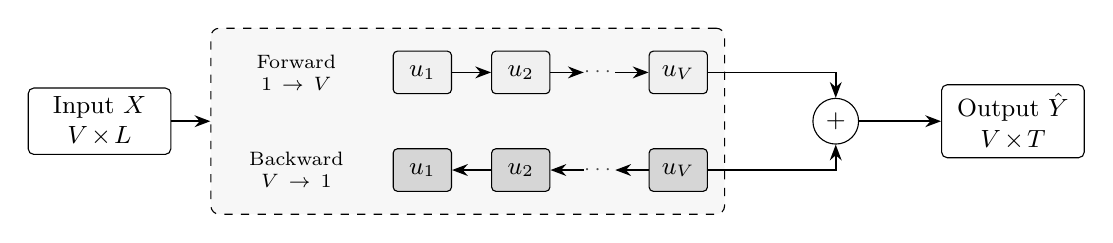
\begin{tikzpicture}[
  font=\small,
  >=Stealth,
  blk/.style={draw, rounded corners=2pt, align=center, inner sep=3pt,
              minimum height=8mm, text width=16mm},
  cell/.style={draw, rounded corners=1.5pt, align=center, inner sep=0pt,
               minimum width=7.4mm, minimum height=5.4mm},
  lab/.style={font=\scriptsize, align=center, text width=15mm},
  arr/.style={->, semithick},
  note/.style={font=\scriptsize, text=black!70}
]
% ---- input ----
\node[blk] (x) at (0.75,0) {Input $X$\\$V\!\times\! L$};

% ---- forward scan: variate axis, 1 -> V ----
\node[lab]  (lf) at (3.25, 0.62) {Forward\\$1\to V$};
\node[cell, fill=black!6]  (f1) at (4.85, 0.62) {$u_1$};
\node[cell, fill=black!6]  (f2) at (6.10, 0.62) {$u_2$};
\node[cell, fill=black!6]  (fV) at (8.10, 0.62) {$u_V$};

% ---- backward scan: variate axis, V -> 1 ----
\node[lab]  (lb) at (3.25,-0.62) {Backward\\$V\to 1$};
\node[cell, fill=black!16] (b1) at (4.85,-0.62) {$u_1$};
\node[cell, fill=black!16] (b2) at (6.10,-0.62) {$u_2$};
\node[cell, fill=black!16] (bV) at (8.10,-0.62) {$u_V$};

% ---- enclosing block (unlabelled) ----
\begin{scope}[on background layer]
\node[draw, dashed, rounded corners=3pt, inner sep=6pt, fill=black!3,
      fit=(lf)(lb)(fV)(bV)] (grp) {};
\end{scope}

% ---- scan directions ----
\draw[arr] (f1.east) -- (f2.west);
\draw[arr] (f2.east) -- (6.90, 0.62);
\node[note, inner sep=1pt] at (7.10, 0.62) {$\cdots$};
\draw[arr] (7.30, 0.62) -- (fV.west);

\draw[arr] (b2.west) -- (b1.east);
\draw[arr] (bV.west) -- (7.30,-0.62);
\node[note, inner sep=1pt] at (7.10,-0.62) {$\cdots$};
\draw[arr] (6.90,-0.62) -- (b2.east);

% ---- fusion and output ----
\node[circle, draw, inner sep=0pt, minimum size=5.8mm] (plus) at (10.1,0) {$+$};
\draw[arr] (x.east) -- (grp.west);
\draw[arr] (fV.east) -| (plus.north);
\draw[arr] (bV.east) -| (plus.south);
\node[blk] (y) at (12.35,0) {Output $\hat{Y}$\\$V\!\times\! T$};
\draw[arr] (plus.east) -- (y.west);
\end{tikzpicture}
\caption{S-Mamba 的双向结构示意图。}
\label{fig:smamba}
\end{figure}

跨变量耦合指的是同一时刻下不同变量之间的相互依赖关系。
在多变量序列中，变量之间通常并不彼此独立，一个变量的取值会携带其他变量的信息，因此模型能否刻画跨变量耦合，决定了它能否利用这些信息。
S-Mamba 的双向扫描沿变量维逐位传递信息，变量间耦合只能被隐式携带于各变量的隐状态之中，模型没有显式环节对它加以刻画。

%% ============================================================
%% QCCK 第三章 中文版
%% 格式参考：Overleaf 项目 6aa379e8fec9886e0960f9e9（article + ctex 单栏中文稿）
%% 内容来源：ch3/第三章修改版1.md（用户中文底稿，逐句原样保留）
%% 处理：去掉「第N句：」写作脚手架；公式排成 equation 环境；
%%       「图 X」引用删除（本版不收录图）；[REF] 落为 bracewell 引用
%% 编译：xelatex（ctex 需要 xelatex 或 lualatex）
%% ============================================================

% [已改造] 本文件现为 main.tex 的分章正文（导言区已并入 main.tex），由 main 统一编译。


\section{QCCK：量子跨变量耦合核}

本章提出量子跨变量耦合核 QCCK，将变量间耦合显式地构造出来。
首先，频域对齐得到去除时移与尺度差异的对齐频谱；随后，QCCE 将变量信息编码为纠缠量子态；
最后，量子核比较各变量量子态的重叠程度，得到可解释的耦合矩阵 $K$，供下游主干在此基础上进行跨变量建模与预测。

\subsection{QCCK 总览}

QCCK 的整体结构由频域对齐、QCCE 与量子核三个环节构成，对每个样本显式度量变量两两之间的耦合，输出可解释的耦合矩阵 $K\in\mathbb{R}^{V\times V}$。
频域对齐作为 QCCK 的输入处理环节，由谱变换与时间轴、频率轴两级对齐构成，将每个变量的原始序列变换为对齐频谱 $S$，消除变量间的时移与周期尺度等环境差异，使耦合度量只刻画变量间的结构关系。对齐频谱 $S$ 是 QCCE 中相位通道的基础。
QCCE 作为 QCCK 方法的核心，通过振幅通道与相位通道将每个变量的信息编码为量子态，并借助参数化量子线路在比特间建立纠缠，构造出能反映数据变量特征的纠缠量子态 $|\psi_v\rangle$，作为量子核度量变量间耦合的输入。
量子核作为 QCCK 的耦合度量环节，以 QCCE 得到的各变量量子态为输入，按式~(\ref{eq:qkernel}) 的保真度核计算任意两个变量 $i$、$j$ 的重叠度作为耦合强度，即 $K[i,j] = |\langle\psi_i|\psi_j\rangle|^2$，其中 $\langle\cdot|\cdot\rangle$ 为 $\mathbb{C}^{32}$ 上的标准内积，$|\psi_i\rangle$、$|\psi_j\rangle$ 分别为变量 $i$、$j$ 经 QCCE 编码得到的量子态。$K\in\mathbb{R}^{V\times V}$ 取值在 $[0,1]$，其每个元素表示一对变量的耦合强度。
因此，$K$ 的可解释性体现在它把变量间的耦合落成一份可检查、可比较的矩阵：据此能定位强耦合的变量对，也能看出单个变量与其余各变量的耦合分布；用热力图呈现会更直观，且每个样本对应一份 $K$，可观察耦合结构随样本的变化。
综上所述，针对现有双向状态空间类主干以扫描方式隐式传递变量间关系、导致变量间耦合难以被显式刻画与利用的问题，我们提出了 QCCK。它显式度量变量间的耦合，得到具备可解释性的耦合矩阵 $K$，把原本隐式的变量间依赖变为可读、可解释的依据。

\subsection{频域对齐}

针对不同变量的波形普遍存在时移与主导周期差异、若不消除会使结构相似的变量被误判为互不相关的问题，为使耦合度量只反映变量间的结构关系，我们提出频域对齐：对每个变量的原始序列进行谱分析，并在时间轴与频率轴上分别消除时移与周期尺度差异，得到对齐频谱 $S$。
对齐后，时移与主导周期的差异不再干扰后续的耦合度量，结构相似而时移、周期不同的变量不会再被误判为互不相关。
记 $V$ 个变量的输入序列为 $x_1,\dots,x_V$，其中 $x_v \in \mathbb{R}^L$ 表示变量 $v$ 在连续 $L$ 个时刻上的原始观测序列，也就是该变量随时间变化的一段数据。这 $V$ 条序列取自同一段连续时刻，共同构成一个样本。我们对每个这样的 $x_v$ 施加实数快速傅里叶变换 rFFT，得到复谱 $X_v(f) \in \mathbb{C}^F$，其中 $F = \lfloor L/2 \rfloor+1$ 为频点个数，$f = 0,1,\dots,F-1$ 为频率索引。
我们定义了幅度谱与相位谱，如公式~(\ref{eq:amp-spec})、(\ref{eq:phase-spec}) 所示，二者分别刻画各频率分量的强度与时间位置。

\textbf{幅度谱。}
\begin{equation}
\label{eq:amp-spec}
A_v(f) = |X_v(f)|.
\end{equation}
$X_v(f)$ 是复数，对它取模 $|X_v(f)|$ 就得到频率 $f$ 分量的幅值，$A_v(f)$ 越大说明该频率成分越强，因此幅度谱刻画各频率分量的强度。当主导周期不同、波形在时间上伸缩时，幅度谱的主峰位置会随之移动，所以尺度差异体现在幅度谱上，频率轴对齐将依据幅度谱的主峰进行。

\textbf{相位谱。}
\begin{equation}
\label{eq:phase-spec}
\phi_v(f) = \arg X_v(f).
\end{equation}
$\arg$ 取复数的辐角，得到频率 $f$ 分量的相位，它决定该分量在时间轴上的起始位置，因此相位谱刻画各频率分量的时间位置。当不同变量的波形存在整体时移时，波形平移改变各分量在时间轴上的起始位置，即改变它们的相位，因此时移差异体现在相位谱上，时间轴对齐将针对相位谱进行。
令 $\hat{f}_{\mathrm{peak}}(v) = \arg\max_{f\geq 1} A_v(f)$ 为幅度谱主频，对应主导周期。忽略直流分量 $f=0$，因为直流只反映序列均值，不对应某个周期。
由尺度定理~\cite{bracewell2000fourier}，时间尺度差异表现为幅度谱~(\ref{eq:amp-spec}) 在频率轴上的缩放，据此归一化频率坐标，如公式~(\ref{eq:freq-align}) 所示：
\begin{equation}
\label{eq:freq-align}
\tilde{f} = f / \hat{f}_{\mathrm{peak}},
\end{equation}
使所有变量的主峰对齐至同一频率位置，消除主导周期差异。
时移校正需要一个共同的时序基准，我们以该样本内除变量 $v$ 外其余变量的平均序列为基准，使基准不受变量 $v$ 自身取值主导。令 $\hat{\delta}_v$ 表示变量 $v$ 相对该基准的时移估计，取为变量 $v$ 与基准互相关峰值对应的滞后占序列长度的比例。
由时移定理~\cite{bracewell2000fourier}，时移差异表现为相位谱~(\ref{eq:phase-spec}) 中随频率线性增长的相位项，据此校正相位谱，如公式~(\ref{eq:time-align}) 所示：
\begin{equation}
\label{eq:time-align}
\phi'_v(f) = \phi_v(f) - 2\pi f\hat{\delta}_v,
\end{equation}
使各变量校正后的相位谱对齐至同一时间原点，仅保留波形自身的结构信息，消除变量间的时移差异。
我们在对齐后的统一频率坐标上取固定的采样区间 $\tilde{f}\in[0,2]$，该区间覆盖主峰 $\tilde{f}=1$ 至其两倍频率以内的谐波结构；在该区间上取 $M = 32$ 个均匀采样点并作线性插值，得重采样幅度谱 $\tilde{A}_v \in \mathbb{R}^M$ 与重采样相位谱 $\tilde{\phi}_v \in \mathbb{R}^M$，拼接为对齐频谱，如公式~(\ref{eq:spectrum}) 所示。
\begin{equation}
\label{eq:spectrum}
S_v = [\,\tilde{A}_v\,;\,\tilde{\phi}_v\,] \in \mathbb{R}^{2M} = \mathbb{R}^{64}.
\end{equation}
由时移定理与尺度定理可知，对齐频谱 $S_v$ 对时移与时间尺度变换保持不变，维度恒为 $2M$，与输入长度 $L$ 无关。
综上所述，频域对齐把每个变量的原始序列变换为对齐频谱 $S_v$，为 QCCE 的相位通道提供同基准的频域输入。

\subsection{QCCE 编码}

编码环节 QCCE 是 QCCK 的重要组成部分，负责把每个变量的信息编码成量子态。它以主干输出的隐状态 $h_v$ 为振幅通道的输入、以频域对齐得到的对齐频谱 $S_v$ 为相位通道的输入，经参数化量子线路在比特间建立纠缠，得到反映变量特征的纠缠量子态 $|\psi_v\rangle$，作为量子核度量变量间耦合的输入。
变量 $v$ 的编码输入有两路：主干隐状态 $h_v\in\mathbb{R}^d$ 与对齐频谱 $S_v\in\mathbb{R}^{2M}$。双向状态空间时序主干把每个变量的整段历史观测编码为 $d$ 维表示并逐层更新，取 QCCK 所在编码层之后变量 $v$ 的表示即得 $h_v$，$h_v$ 刻画该变量自身的时序特征。对齐频谱由频域对齐从变量 $v$ 的原始序列得到，携带各频率成分对齐后的强度与相位信息。
为解决两类异质输入要进入同一个量子态且互不干扰的问题，我们定义了振幅通道与相位通道。
振幅通道把变量自身特征编码为各计算基态的概率：它以 $h_v$ 为输入，设振幅投影矩阵 $W_r\in\mathbb{R}^{32\times d}$，令
\begin{equation}
\label{eq:amp-channel}
p(h_v) = \mathrm{softmax}(W_r\cdot h_v) \in \mathbb{R}^{32}.
\end{equation}
$p(h_v)$ 各分量非负且和为 1，给出各计算基态被选中的概率。
相位通道把对齐频谱编码为各基态的相位：它以 $S_v$ 为输入，设相位投影矩阵 $W_\theta\in\mathbb{R}^{32\times 2M}$，令
\begin{equation}
\label{eq:phase-channel}
\theta(S_v) = W_\theta\cdot S_v \in \mathbb{R}^{32}.
\end{equation}
$\theta(S_v)$ 各分量给出对应计算基态的相位。
两个通道由此各司其职：振幅通道给出的概率决定各基态的振幅，相位通道给出的相位决定各基态间的相对相位；由于振幅与相位是量子态相互独立的两个自由度，两类信息互不干扰，使合成的量子态能够同时携带变量自身特征与频域信息。振幅、相位两通道的投影矩阵以及参数化线路的旋转角均对每个变量独立可学习，公式为行文简洁省略变量下标。
记 $b\in\{0,1\}^5$ 为 5 个量子比特的基态标记，$|b\rangle$ 为对应计算基态，共 $2^5=32$ 个；$p_b(h_v)$、$\theta_b(S_v)$ 分别为 $p(h_v)$、$\theta(S_v)$ 的第 $b$ 个分量，给出基态 $|b\rangle$ 的概率与相位。我们把这 32 个基态按各自的概率与相位叠加，即得变量 $v$ 在进入量子线路前的编码态
\begin{equation}
\label{eq:encode}
|\chi_v\rangle = \sum_{b\in\{0,1\}^5} \sqrt{p_b(h_v)} \cdot e^{\,i\cdot\theta_b(S_v)} \cdot |b\rangle.
\end{equation}
至此，变量 $v$ 的编码态 $|\chi_v\rangle$ 构造完成，作为变量 $v$ 进入后续量子线路演化的输入。式~(\ref{eq:encode}) 是式~(\ref{eq:joint-encoding}) 的联合编码在本文中的具体形式：振幅由主干隐状态给出，相位由对齐频谱给出。
为使编码态在比特间引入纠缠、得到量子核度量耦合所用的纠缠量子态，我们让编码态 $|\chi_v\rangle$ 经参数化量子线路演化。每个变量沿各自独立可学习的线路演化，变量 $v$ 的线路酉记作 $U_v$，一层由 RY、RZ 旋转门与 CNOT 纠缠门构成，其算符形式为
\begin{equation}
\label{eq:circuit}
U_v = \mathrm{CNOT}_{4,5}\cdot\mathrm{CNOT}_{3,4}\cdot\mathrm{CNOT}_{2,3}\cdot\mathrm{CNOT}_{1,2} \cdot \Bigl(\bigotimes_{q=1}^{5} RZ_q(\beta_q)\cdot RY_q(\alpha_q)\Bigr),
\end{equation}
其中 CNOT 依次作用于相邻比特对 $(1,2)$、$(2,3)$、$(3,4)$、$(4,5)$；$\alpha_q$、$\beta_q$ 为变量 $v$ 线路的可学习旋转角。式中 $R_Y$、$R_Z$ 旋转门与 CNOT 纠缠门的定义见附录~\ref{app:quantum}。编码态连续经过两层相同的 $U_v$，得到变量 $v$ 的最终量子态
\begin{equation}
\label{eq:final-state}
|\psi_v\rangle = U_v\cdot U_v\cdot|\chi_v\rangle.
\end{equation}
$|\psi_v\rangle$ 是变量 $v$ 的量子态表示：主干隐状态 $h_v$ 经振幅通道写成各计算基态的概率，对齐频谱 $S_v$ 经相位通道写成基态间的相位，两层线路又在比特间引入纠缠。它把主干隐状态 $h_v$ 与对齐频谱 $S_v$ 这两类异质输入收进同一个单位向量，每个变量各得一个 $|\psi_v\rangle$、构造一致，是连接编码输入与后续耦合度量的枢纽。
本节完成 QCCK 的编码环节 QCCE：以主干隐状态与对齐频谱为输入，经振幅、相位两个通道分别承载变量自身特征与频域信息，再经参数化量子线路两层的演化，把每个变量编码为一个归一化的纠缠量子态 $|\psi_v\rangle$。下一步，量子核将基于这些量子态度量变量间的耦合。

\subsection{量子核}

量子核作为 QCCK 的耦合度量环节，负责度量变量两两之间的耦合强度。它以各变量经 QCCE 编码并演化得到的纠缠量子态 $|\psi_v\rangle$ 为输入，对样本中的任意两个变量计算两态的重叠程度，得到耦合矩阵 $K\in\mathbb{R}^{V\times V}$。
变量 $i$、$j$ 的耦合强度由二者的量子态共同决定。量子核按式~(\ref{eq:qkernel}) 计算两态的重叠度，即内积模长的平方 $|\langle\psi_i|\psi_j\rangle|^2$，其中 $\langle\cdot|\cdot\rangle$ 为 $\mathbb{C}^{32}$ 上的标准内积，$|\psi_i\rangle$、$|\psi_j\rangle$ 分别为变量 $i$、$j$ 经 QCCE 编码并演化得到的纠缠量子态。
两量子态的重叠度即二者的保真度，因此本文采用的耦合度量就是式~(\ref{eq:qkernel}) 给出的保真度核。
保真度核刻画两态的重叠程度：两态越接近，输出越接近 1；两态越趋于正交，输出越接近 0；
当两变量为同一变量时，量子态与自身完全重叠，输出恒为 1，所以耦合矩阵的对角元素恒为 1。
综上，QCCK 以原始序列与主干隐状态为输入，经频域对齐、QCCE 与量子核三个环节，显式度量变量间的耦合，得到耦合矩阵 $K\in\mathbb{R}^{V\times V}$。$K$ 中任意两个变量的耦合强度都能直接读取，配合热力图即可定位强耦合的变量对，耦合关系因此不会隐没于黑盒权重之中。
可解释性由此随度量一同产生，模型所依据的变量间关系都能通过该矩阵直接呈现与核对。
在此基础上，第四章进一步将 QCCK 以 QCCK Layer 的形式嵌入状态空间主干的编码器层之间，并利用耦合矩阵 $K$ 引导跨变量信息融合，使显式度量得到的耦合关系直接参与变量表示更新与预测。




%% ============================================================
%% QCCK-M 第四章 中文版
%% 格式参考：Overleaf 项目 6aa379e8fec9886e0960f9e9（article + ctex 单栏中文稿）
%% 内容来源：ch4/第四章修改2.md（用户中文底稿，逐句原样保留）
%% 处理：去掉「第N句：」写作脚手架；公式排成 equation 环境；
%%       「图 X」引用删除；算法块排成 algorithm 环境
%% 编译：xelatex（ctex 需要 xelatex 或 lualatex）
%% ============================================================

% [已改造] 本文件现为 main.tex 的分章正文（导言区已并入 main.tex），由 main 统一编译。


\section{QCCK-M：面向多变量时间序列预测的量子跨变量耦合网络}

第三章提出 QCCK，将变量间的耦合显式度量为可解释的耦合矩阵 $K$。然而，耦合矩阵只有参与变量表示更新，才能进一步作用于预测过程。
为此，本章将 QCCK 以 QCCK Layer 的形式嵌入编码器层之间，构成完整的预测网络 QCCK-M，使显式耦合能够参与跨变量信息融合。
4.1 给出 QCCK-M 的整体结构与数据流，4.2 给出单个 QCCK Layer 的前向算法与网络训练细节。

\subsection{QCCK-M 总览}

QCCK-M 的整体结构与数据流如下：输入的多变量时序数据经 RevIN 与 Tokenize 预处理，成为每个变量的 $d$ 维表示 token；时序主干编码器逐层更新这些 token，QCCK Layer 则嵌入每个编码器层之后，根据显式度量的耦合进行一次跨变量混合；最后经预测头映射并反归一化，输出各变量的预测 $\hat{Y}$。
RevIN 与 Tokenize 是 QCCK-M 的输入预处理环节。
RevIN 把每个变量沿时间轴减去均值、除以标准差，以缓解样本间的分布漂移.
Tokenize 用一个线性层把每个变量的整段历史观测编码为一个 $d$ 维的变量 token。
变量 token 连同提供时间上下文的时间特征 token 一并作为主干编码器的输入。
主干编码器逐层更新变量 token，每个编码器层在层末输出所有变量的隐状态 $H\in\mathbb{R}^{B\times V\times d}$。
主干编码器层通过双向状态空间扫描实现变量间的信息交互，但该交互过程并不显式输出变量两两之间的耦合关系。
为使第三章得到的显式耦合参与每层变量表示更新，QCCK-M 在每个编码器层之后引入一个 QCCK Layer。
QCCK Layer 以该层的隐状态 $H$ 与对齐频谱 $S$ 为输入，把各变量经 QCCE 编码成量子态，用保真度核度量变量两两之间的耦合，得到耦合矩阵 $K$.随后，$K$ 经去除对角自耦合后直接用于跨变量消息聚合，每个变量依据显式耦合强度接收其他变量的信息，并通过残差方式写回，得到融合跨变量信息的更新隐状态 $H'$。
预测头把每个变量的最终隐状态线性映射为长度等于预测长度的预测序列，并经反归一化还原到原始尺度，得到各变量的预测 $\hat{Y}$。
完成前向预测后，QCCK-M 以时域误差与频域监督项之和作为训练目标，并对整网进行端到端优化，损失函数的具体形式见 4.2。
综上，QCCK-M 通过在主干的逐层表示更新过程中引入 QCCK，使显式度量得到的耦合矩阵 $K$ 成为跨变量信息融合的依据。
因此，$K$ 直接参与变量表示更新，同时以显式矩阵形式保留，可用于检查变量间的耦合关系。单个 QCCK Layer 的前向算法与网络训练细节见 4.2。

\subsection{QCCK-M 的算法}

QCCK-M 在每个主干编码器层之后插入结构相同的 QCCK Layer，各层共享由输入序列得到的对齐频谱 $S$，因此本节先给出单个 QCCK Layer 的前向过程，再说明整网的训练目标与参数设置。

\begin{algorithm}[htbp]
\caption{QCCK Layer 前向传播}
\label{alg:qcck-layer-zh}
\begin{algorithmic}[1]
\REQUIRE 主干隐状态 $H\in\mathbb{R}^{B\times V\times d}$，对齐频谱 $S\in\mathbb{R}^{B\times V\times 2M}$
\ENSURE 更新后的隐状态 $H'$，耦合矩阵 $K$
\STATE 对每个变量 $v$，由 QCCE 构造量子态，经两层 $U_v$ 演化得到 $|\psi_v\rangle$
\STATE 计算保真度核 $K[i,j] = |\langle\psi_i|\psi_j\rangle|^2$
\STATE 去除自耦合：$K \leftarrow K - I$
\STATE 消息投影：$H_q = H \cdot W_q$
\STATE 跨变量聚合：$H_p = K \cdot H_q$
\STATE 残差更新：$H' = \mathrm{LN}(H + \gamma \cdot H_p)$
\RETURN $H'$, $K$
\end{algorithmic}
\end{algorithm}

算法第 1、2 步复用第三章定义的 QCCE 与保真度核。
每个变量 $v$ 由当前层隐状态 $h_v$ 与共享对齐频谱 $S_v$ 构造量子态，并经参数化量子线路 $U_v$ 演化得到 $|\psi_v\rangle$；变量 $i$ 与变量 $j$ 的耦合强度由式~(\ref{eq:qkernel}) 的保真度 $K[i,j] = |\langle\psi_i|\psi_j\rangle|^2$ 给出。
本文固定使用 5 个量子比特，因此每个变量的量子态位于 32 维复 Hilbert 空间。
算法第 3 步用于去除变量自身耦合。
由于保真度核的对角元素恒为 1，即 $K[i,i]=1$，该部分仅表示变量自身相似性，而非跨变量关系。
因此，本文将对角元素置零，仅保留变量之间的耦合信息用于后续跨变量传播。
算法第 4 至 5 步完成消息生成与跨变量融合。
每个变量的隐状态先经可学习投影 $W_q$ 得到消息表示 $H_q$，再由耦合矩阵 $K$ 对不同变量消息进行加权聚合，得到跨变量表示 $H_p$。
由于 $K$ 中每个元素直接对应变量间耦合强度，因此强耦合变量能够贡献更多跨变量信息，而弱耦合变量的影响自然受到抑制。
算法第 6 步通过残差结构完成变量表示更新。
其中，$\gamma$ 为可学习融合系数，用于控制 QCCK Layer 对原始主干表示的注入强度。
通过残差连接，模型能够在保留主干已学习时间模式的同时，引入由量子耦合关系提供的跨变量信息。
量子核需要计算变量两两之间的量子态保真度，其计算复杂度为 $O(V^2\cdot 2^N)$，其中 $V$ 为变量数，$N$ 为量子比特数。
本文固定 $N=5$，因此量子态维度为 32，且该计算不随输入序列长度 $L$ 增长。
QCCK-M 采用时域监督与频域监督联合训练，整体训练目标为：
\begin{equation}
\label{eq:loss-zh}
L = L_{\mathrm{time}} + \lambda \cdot L_{\mathrm{FreDF}},
\end{equation}
其中
\begin{equation}
L_{\mathrm{time}} = \lVert \hat{Y} - Y \rVert^2
\end{equation}
用于约束预测序列与真实序列在时域上的误差；
\begin{equation}
L_{\mathrm{FreDF}} = \mathrm{mean}\,\lvert \mathrm{rFFT}(\hat{Y}) - \mathrm{rFFT}(Y) \rvert
\end{equation}
用于约束二者在频域表示上的差异，$\lambda$ 为频域监督项的权重。
QCCE、参数化量子线路、QCCK Layer 与时序主干中的可学习参数均由上述联合损失进行端到端优化。
QCCK-M 保留主干原有的编码器与预测头结构，仅在编码器层之间引入 QCCK Layer，并增加频域监督项。



%% ============================================================
%% QCCK-M 第五章（实验）中文版
%% 格式参考：Overleaf 项目 6aa379e8fec9886e0960f9e9（article + ctex 单栏中文稿）
%% 内容来源：ch5/ch5cn_pdf.py（原 ReportLab 版），由 ch5/gen_ch5tex.py 程序化转换，
%%           正文逐句原样保留；表格按原脚本同一套数据与排名逻辑重算。
%% 编译：xelatex（ctex 需要 xelatex 或 lualatex），跑两遍
%% 图：\ifchfivefigs 开关控制。本地全版=true；推 Overleaf（纯文字、不带图）改 false。
%% ============================================================

% [已改造] 本文件现为 main.tex 的分章正文（导言区已并入 main.tex），由 main 统一编译。



\section{实验}

\subsection{A　实验配置与主结果}

本章在九个多变量时序数据集上验证 QCCK-M。
A 节给出实验配置与主结果，B 节用消融分离量子核与频域监督两组件的贡献，C 节用输入扰动实验检验主干是否真正利用了跨变量信息，D 节给出耦合矩阵的可解释性结果。
我们在一组多变量时序数据集上评估 QCCK-M。
在 ETT 家族\cite{zhou2021informer}的 ETTh1、ETTh2、ETTm1、ETTm2，以及 Weather、ECL、Traffic、Exchange 八个常用基准\cite{wu2021autoformer}之上，我们还加入  Beijing-AQI 这个七变量的单站空气质量数据集，用它代表同一站点的多通道物理系统。
表 1 给出各数据集的变量数与观测数。
这些数据覆盖不同的变量耦合形态，包括站点级物理系统、气象观测、大量独立电表、交通传感器网络与汇率序列。按照主干基线的惯例，输入长度取 96，报告四个预测长度 96、192、336、720。数据划分遵循各基准的原始协议：ETT 家族的四个数据集按 12 个月、4 个月、4 个月划分为训练、验证与测试三份，Weather、ECL、Traffic、Exchange 与 Beijing-AQI 按时间顺序以 7 比 1 比 2 的比例划分。
评测指标取反归一化之后的 MSE 与 MAE，同一行的两个指标来自同一次测试运行。

%我们以 S-Mamba[1] 为主干，在其编码器层之间插入耦合模块，得到 QCCK-M。(文章要避免这种预言描述，这样的描述会让人觉得你的工作就是 S-Mamba导致没有创新，也就是说当你后面改论文的时候出现 S-Mamba 就一定要慎重 如果不是超越他就不要写)
每一条基线都使用其公开发布的实现与论文推荐的配置。
对比主干按其官方脚本在本机复现，表 2 中对应列即本机复现值。
iTransformer、DLinear、PatchTST、TimesNet、SAMBA、CMamba、Affirm 与 DeMa 在统一的长时序评测框架下，以各自的公开实现与默认配置复现，全部方法在同一划分、同一输入长度与同一指标口径下比较。
逐条而言，iTransformer\cite{liu2024itransformer} 把自注意力作用在变量维，DLinear\cite{zeng2023dlinear} 以分解加线性取胜，PatchTST\cite{nie2023patchtst} 采用分块与通道独立，TimesNet\cite{wu2023timesnet} 挖掘多周期结构，CMamba 与 SAMBA 属于 Mamba\cite{gu2024mamba} 状态空间家族，Affirm 与 DeMa\cite{an2026dema} 为近期的 Transformer 预测方法。所有模型用 PyTorch 实现，实验在 8 张 NVIDIA RTX 4090 GPU 上完成。
对每一条基线，我们采用其公开发布的模型结构与官方推荐的超参数。对我们提出的 QCCK-M，我们在验证集上对量子比特数与学习率做小范围网格搜索，以确定一组默认配置。
训练按验证损失早停；对两个最大的数据集，主干编码维度与对比主干的官方实现对齐到 512，避免把增益误归于模型规模。我们提出的 QCCK-M 在时域 MSE 之上加入频域监督项\cite{wang2025fredf}，该项权重取 1.0。
量子核采用固定配置；所有耦合分析均基于原始保真度核 f。主结果将 QCCK-M 与双向状态空间主干基线以及八条近期基线对比，这些基线覆盖主要技术路线，包括 Mamba 与状态空间族的 CMamba 与 SAMBA，Transformer 族的 iTransformer、PatchTST、Affirm 与 DeMa，多尺度卷积模型 TimesNet，以及线性模型 DLinear。

\begin{center}

\begin{minipage}{\textwidth}

\footnotesize

表 1　各数据集的变量数与观测数。ETT 家族为站点级电力负荷，Weather 为气象站观测，ECL 与 Traffic 分别为电表与交通传感器网络，Exchange 为汇率，Beijing-AQI 为单站空气质量。\\[2pt]

\centering

\setlength{\tabcolsep}{4pt}

\begin{tabular}{@{}lcc@{}}

\hline

数据集 & 变量数 & 观测数 \\ \hline

ETTh1 & 7 & 17,420 \\

ETTh2 & 7 & 17,420 \\

ETTm1 & 7 & 69,680 \\

ETTm2 & 7 & 69,680 \\

Weather & 21 & 52,696 \\

ECL & 321 & 26,304 \\

Traffic & 862 & 17,544 \\

Exchange & 8 & 7,587 \\

Beijing-AQI & 7 & 23,050 \\

\hline

\end{tabular}

\end{minipage}

\end{center}

表 2 系列逐数据集汇总 QCCK-M 与各基线方法。在全部 36 个设置上，QCCK-M 在其中 34 个设置取得比 S-Mamba 更低的 MSE，其余两个设置即 Exchange 在 720 与 Traffic 在 336 与之基本持平。在站点级多变量系统上增益稳定为正，例如 ETTh1 的 96 步提升 3.4\%，ETTm2 的 96 步提升 6.2\%，Beijing 各步的提升在 3\% 到 11\% 之间。在变量数量大而耦合偏弱的数据集上，主干容量对齐之后仍取得正的增益，只是幅度较小。
与八条经典基线相比，QCCK-M 在 ETTh2、ETTm2、ECL、Traffic 与 Beijing 这些核心多变量数据集的全部格点上优于八条基线，在其余数据集上保持竞争力，通常与最强基线的差距在千分之几以内。表中的每个格子都同时给出 MSE 与 MAE，两数来自同一次运行。

\clearpage

\fontsize{6.2}{7.2}\selectfont

表 2　主结果。行按数据集与预测长度展开，列为各模型；每个格子的上一行为 MSE、下一行为 MAE，两数来自同一次运行。同一行内 MSE 与 MAE 各自独立排名：最优者以灰底加粗标出，次优者以浅灰底标出。

\setlength{\tabcolsep}{2.2pt}

\renewcommand{\arraystretch}{0.62}

\setlength{\fboxsep}{0.5pt}

\begin{longtable}{@{}llcccccccccc@{}}
\hline
数据集 & H & QCCK-M & S-Mamba & iTransformer & DLinear & PatchTST & TimesNet & SAMBA & CMamba & Affirm & DeMa \\ \hline
\endfirsthead
\hline
数据集 & H & QCCK-M & S-Mamba & iTransformer & DLinear & PatchTST & TimesNet & SAMBA & CMamba & Affirm & DeMa \\ \hline
\endhead
\hline \multicolumn{12}{r}{（续下页）} \\
\endfoot
\hline
\endlastfoot

\textbf{ETTh1} & 96 & \shortstack{\colorbox[gray]{0.82}{\textbf{0.3745}}\\\colorbox[gray]{0.82}{\textbf{0.3971}}} & \shortstack{0.3877\\0.4064} & \shortstack{0.3950\\0.4098} & \shortstack{0.3962\\0.4108} & \shortstack{\colorbox[gray]{0.92}{0.3796}\\\colorbox[gray]{0.92}{0.3992}} & \shortstack{0.3890\\0.4120} & \shortstack{0.3896\\0.4050} & \shortstack{0.3889\\0.4066} & \shortstack{0.4009\\0.4149} & \shortstack{0.3965\\0.4133} \\ \cline{2-12}

 & 192 & \shortstack{\colorbox[gray]{0.82}{\textbf{0.4255}}\\\colorbox[gray]{0.82}{\textbf{0.4271}}} & \shortstack{0.4450\\0.4407} & \shortstack{0.4486\\0.4412} & \shortstack{0.4450\\0.4404} & \shortstack{\colorbox[gray]{0.82}{\textbf{0.4255}}\\\colorbox[gray]{0.92}{0.4316}} & \shortstack{\colorbox[gray]{0.92}{0.4394}\\0.4417} & \shortstack{0.4477\\0.4392} & \shortstack{0.4444\\0.4400} & \shortstack{0.4608\\0.4486} & \shortstack{0.4571\\0.4488} \\ \cline{2-12}

 & 336 & \shortstack{\colorbox[gray]{0.82}{\textbf{0.4678}}\\\colorbox[gray]{0.82}{\textbf{0.4489}}} & \shortstack{0.4904\\0.4653} & \shortstack{0.4921\\0.4654} & \shortstack{0.4874\\0.4654} & \shortstack{\colorbox[gray]{0.92}{0.4703}\\\colorbox[gray]{0.92}{0.4577}} & \shortstack{0.4952\\0.4714} & \shortstack{0.4971\\0.4669} & \shortstack{0.4919\\0.4670} & \shortstack{0.5193\\0.4800} & \shortstack{0.5259\\0.4868} \\ \cline{2-12}

 & 720 & \shortstack{\colorbox[gray]{0.82}{\textbf{0.4833}}\\\colorbox[gray]{0.82}{\textbf{0.4849}}} & \shortstack{\colorbox[gray]{0.92}{0.5066}\\0.4966} & \shortstack{0.5215\\0.5041} & \shortstack{0.5126\\0.5104} & \shortstack{0.5211\\0.5065} & \shortstack{0.5189\\0.4944} & \shortstack{0.5107\\\colorbox[gray]{0.92}{0.4939}} & \shortstack{0.5119\\0.5005} & \shortstack{0.5850\\0.5318} & \shortstack{0.5749\\0.5298} \\ \hline

\textbf{ETTh2} & 96 & \shortstack{\colorbox[gray]{0.82}{\textbf{0.2849}}\\\colorbox[gray]{0.82}{\textbf{0.3367}}} & \shortstack{0.2971\\0.3486} & \shortstack{0.3004\\0.3496} & \shortstack{0.3414\\0.3953} & \shortstack{0.2978\\0.3473} & \shortstack{0.3370\\0.3709} & \shortstack{\colorbox[gray]{0.92}{0.2968}\\\colorbox[gray]{0.92}{0.3470}} & \shortstack{0.2975\\0.3493} & \shortstack{0.3090\\0.3592} & \shortstack{0.3059\\0.3557} \\ \cline{2-12}

 & 192 & \shortstack{\colorbox[gray]{0.82}{\textbf{0.3646}}\\\colorbox[gray]{0.82}{\textbf{0.3886}}} & \shortstack{\colorbox[gray]{0.92}{0.3767}\\0.3988} & \shortstack{0.3818\\0.3998} & \shortstack{0.4819\\0.4792} & \shortstack{0.3813\\0.4044} & \shortstack{0.4046\\0.4146} & \shortstack{0.3784\\\colorbox[gray]{0.92}{0.3985}} & \shortstack{0.3792\\0.4000} & \shortstack{0.3885\\0.4067} & \shortstack{0.3830\\0.4023} \\ \cline{2-12}

 & 336 & \shortstack{\colorbox[gray]{0.82}{\textbf{0.4002}}\\\colorbox[gray]{0.82}{\textbf{0.4170}}} & \shortstack{0.4248\\0.4351} & \shortstack{0.4236\\\colorbox[gray]{0.92}{0.4324}} & \shortstack{0.5929\\0.5422} & \shortstack{0.4227\\0.4378} & \shortstack{0.4565\\0.4523} & \shortstack{0.4264\\0.4357} & \shortstack{\colorbox[gray]{0.92}{0.4222}\\0.4330} & \shortstack{0.4302\\0.4409} & \shortstack{0.4276\\0.4395} \\ \cline{2-12}

 & 720 & \shortstack{\colorbox[gray]{0.82}{\textbf{0.4084}}\\\colorbox[gray]{0.82}{\textbf{0.4333}}} & \shortstack{0.4396\\0.4484} & \shortstack{\colorbox[gray]{0.92}{0.4264}\\\colorbox[gray]{0.92}{0.4451}} & \shortstack{0.8403\\0.6611} & \shortstack{0.4355\\0.4546} & \shortstack{0.4340\\0.4480} & \shortstack{0.4312\\0.4489} & \shortstack{0.4376\\0.4491} & \shortstack{0.4377\\0.4528} & \shortstack{0.4379\\0.4534} \\ \hline

\textbf{ETTm1} & 96 & \shortstack{\colorbox[gray]{0.82}{\textbf{0.3180}}\\\colorbox[gray]{0.82}{\textbf{0.3554}}} & \shortstack{0.3302\\0.3677} & \shortstack{0.3413\\0.3764} & \shortstack{0.3459\\0.3737} & \shortstack{\colorbox[gray]{0.92}{0.3276}\\0.3670} & \shortstack{0.3339\\0.3754} & \shortstack{0.3312\\\colorbox[gray]{0.92}{0.3662}} & \shortstack{0.3317\\0.3663} & \shortstack{0.3332\\0.3685} & \shortstack{0.3368\\0.3706} \\ \cline{2-12}

 & 192 & \shortstack{\colorbox[gray]{0.82}{\textbf{0.3661}}\\\colorbox[gray]{0.82}{\textbf{0.3808}}} & \shortstack{0.3770\\0.3935} & \shortstack{0.3806\\0.3949} & \shortstack{0.3818\\0.3911} & \shortstack{\colorbox[gray]{0.92}{0.3706}\\\colorbox[gray]{0.92}{0.3909}} & \shortstack{0.4085\\0.4138} & \shortstack{0.3866\\0.3985} & \shortstack{0.3826\\0.3954} & \shortstack{0.3888\\0.3996} & \shortstack{0.3809\\0.3952} \\ \cline{2-12}

 & 336 & \shortstack{\colorbox[gray]{0.92}{0.4023}\\\colorbox[gray]{0.82}{\textbf{0.4068}}} & \shortstack{0.4128\\0.4144} & \shortstack{0.4191\\0.4189} & \shortstack{0.4153\\0.4150} & \shortstack{\colorbox[gray]{0.82}{\textbf{0.3984}}\\\colorbox[gray]{0.92}{0.4085}} & \shortstack{0.4158\\0.4224} & \shortstack{0.4259\\0.4235} & \shortstack{0.4223\\0.4217} & \shortstack{0.4267\\0.4241} & \shortstack{0.4337\\0.4293} \\ \cline{2-12}

 & 720 & \shortstack{\colorbox[gray]{0.92}{0.4727}\\\colorbox[gray]{0.92}{0.4493}} & \shortstack{0.4741\\0.4513} & \shortstack{0.4863\\0.4556} & \shortstack{0.4730\\0.4509} & \shortstack{\colorbox[gray]{0.82}{\textbf{0.4602}}\\\colorbox[gray]{0.82}{\textbf{0.4464}}} & \shortstack{0.4827\\0.4589} & \shortstack{0.5075\\0.4671} & \shortstack{0.4855\\0.4568} & \shortstack{0.5051\\0.4656} & \shortstack{0.4989\\0.4627} \\ \hline

\textbf{ETTm2} & 96 & \shortstack{\colorbox[gray]{0.82}{\textbf{0.1704}}\\\colorbox[gray]{0.82}{\textbf{0.2515}}} & \shortstack{0.1817\\0.2661} & \shortstack{0.1838\\0.2669} & \shortstack{0.1934\\0.2928} & \shortstack{0.1829\\0.2678} & \shortstack{0.1896\\0.2665} & \shortstack{\colorbox[gray]{0.92}{0.1804}\\\colorbox[gray]{0.92}{0.2648}} & \shortstack{0.1864\\0.2723} & \shortstack{0.1838\\0.2683} & \shortstack{0.1832\\0.2682} \\ \cline{2-12}

 & 192 & \shortstack{\colorbox[gray]{0.82}{\textbf{0.2387}}\\\colorbox[gray]{0.82}{\textbf{0.2959}}} & \shortstack{0.2510\\0.3126} & \shortstack{0.2528\\0.3125} & \shortstack{0.2845\\0.3614} & \shortstack{\colorbox[gray]{0.92}{0.2466}\\\colorbox[gray]{0.92}{0.3068}} & \shortstack{0.2524\\0.3071} & \shortstack{0.2504\\0.3107} & \shortstack{0.2512\\0.3119} & \shortstack{0.2523\\0.3116} & \shortstack{0.2522\\0.3118} \\ \cline{2-12}

 & 336 & \shortstack{\colorbox[gray]{0.82}{\textbf{0.3022}}\\\colorbox[gray]{0.82}{\textbf{0.3375}}} & \shortstack{\colorbox[gray]{0.92}{0.3115}\\0.3495} & \shortstack{0.3150\\0.3515} & \shortstack{0.3849\\0.4295} & \shortstack{0.3151\\0.3514} & \shortstack{0.3208\\\colorbox[gray]{0.92}{0.3490}} & \shortstack{0.3138\\0.3501} & \shortstack{0.3129\\0.3494} & \shortstack{0.3183\\0.3532} & \shortstack{0.3169\\0.3523} \\ \cline{2-12}

 & 720 & \shortstack{\colorbox[gray]{0.82}{\textbf{0.4077}}\\\colorbox[gray]{0.82}{\textbf{0.3976}}} & \shortstack{\colorbox[gray]{0.92}{0.4110}\\\colorbox[gray]{0.92}{0.4050}} & \shortstack{0.4119\\0.4060} & \shortstack{0.5561\\0.5235} & \shortstack{0.4200\\0.4128} & \shortstack{0.4193\\0.4055} & \shortstack{0.4121\\0.4054} & \shortstack{0.4159\\0.4088} & \shortstack{0.4264\\0.4151} & \shortstack{0.4235\\0.4121} \\ \hline

\textbf{Weather} & 96 & \shortstack{\colorbox[gray]{0.82}{\textbf{0.1581}}\\\colorbox[gray]{0.82}{\textbf{0.1997}}} & \shortstack{\colorbox[gray]{0.92}{0.1649}\\\colorbox[gray]{0.92}{0.2090}} & \shortstack{0.1753\\0.2159} & \shortstack{0.1962\\0.2561} & \shortstack{0.1761\\0.2172} & \shortstack{0.1690\\0.2195} & \shortstack{0.1707\\0.2128} & \shortstack{0.1709\\0.2134} & \shortstack{0.1673\\0.2112} & \shortstack{0.1667\\0.2117} \\ \cline{2-12}

 & 192 & \shortstack{\colorbox[gray]{0.82}{\textbf{0.2092}}\\\colorbox[gray]{0.82}{\textbf{0.2476}}} & \shortstack{\colorbox[gray]{0.92}{0.2154}\\0.2547} & \shortstack{0.2252\\0.2578} & \shortstack{0.2389\\0.2992} & \shortstack{0.2213\\0.2566} & \shortstack{0.2254\\0.2651} & \shortstack{0.2177\\0.2559} & \shortstack{0.2186\\0.2563} & \shortstack{0.2173\\0.2558} & \shortstack{0.2157\\\colorbox[gray]{0.92}{0.2546}} \\ \cline{2-12}

 & 336 & \shortstack{\colorbox[gray]{0.82}{\textbf{0.2680}}\\\colorbox[gray]{0.82}{\textbf{0.2918}}} & \shortstack{\colorbox[gray]{0.92}{0.2729}\\\colorbox[gray]{0.92}{0.2961}} & \shortstack{0.2796\\0.2981} & \shortstack{0.2811\\0.3306} & \shortstack{0.2795\\0.2969} & \shortstack{0.2815\\0.3037} & \shortstack{0.2745\\0.2981} & \shortstack{0.2762\\0.2989} & \shortstack{0.2751\\0.2985} & \shortstack{0.2745\\0.2987} \\ \cline{2-12}

 & 720 & \shortstack{\colorbox[gray]{0.92}{0.3483}\\\colorbox[gray]{0.82}{\textbf{0.3444}}} & \shortstack{0.3531\\0.3489} & \shortstack{0.3611\\0.3510} & \shortstack{\colorbox[gray]{0.82}{\textbf{0.3454}}\\0.3819} & \shortstack{0.3586\\\colorbox[gray]{0.92}{0.3483}} & \shortstack{0.3597\\0.3547} & \shortstack{0.3529\\0.3487} & \shortstack{0.3554\\0.3494} & \shortstack{0.3546\\0.3509} & \shortstack{0.3535\\0.3508} \\ \hline

\textbf{ECL} & 96 & \shortstack{\colorbox[gray]{0.82}{\textbf{0.1341}}\\\colorbox[gray]{0.82}{\textbf{0.2301}}} & \shortstack{\colorbox[gray]{0.92}{0.1387}\\\colorbox[gray]{0.92}{0.2359}} & \shortstack{0.1483\\0.2400} & \shortstack{0.2104\\0.3016} & \shortstack{0.1801\\0.2730} & \shortstack{0.1679\\0.2716} & \shortstack{0.1437\\0.2402} & \shortstack{0.1500\\0.2540} & \shortstack{0.1434\\0.2395} & \shortstack{0.1429\\0.2392} \\ \cline{2-12}

 & 192 & \shortstack{\colorbox[gray]{0.82}{\textbf{0.1541}}\\\colorbox[gray]{0.82}{\textbf{0.2492}}} & \shortstack{0.1610\\0.2582} & \shortstack{0.1644\\\colorbox[gray]{0.92}{0.2557}} & \shortstack{0.2102\\0.3047} & \shortstack{0.1874\\0.2796} & \shortstack{0.1861\\0.2884} & \shortstack{0.1605\\0.2565} & \shortstack{0.1661\\0.2670} & \shortstack{0.1640\\0.2579} & \shortstack{\colorbox[gray]{0.92}{0.1597}\\0.2560} \\ \cline{2-12}

 & 336 & \shortstack{\colorbox[gray]{0.82}{\textbf{0.1733}}\\\colorbox[gray]{0.82}{\textbf{0.2665}}} & \shortstack{0.1803\\0.2771} & \shortstack{\colorbox[gray]{0.92}{0.1779}\\\colorbox[gray]{0.92}{0.2707}} & \shortstack{0.2231\\0.3192} & \shortstack{0.2042\\0.2959} & \shortstack{0.2025\\0.3041} & \shortstack{0.1810\\0.2777} & \shortstack{0.1878\\0.2878} & \shortstack{0.1790\\0.2726} & \shortstack{0.1800\\0.2770} \\ \cline{2-12}

 & 720 & \shortstack{\colorbox[gray]{0.82}{\textbf{0.1913}}\\\colorbox[gray]{0.82}{\textbf{0.2869}}} & \shortstack{\colorbox[gray]{0.92}{0.2046}\\\colorbox[gray]{0.92}{0.2992}} & \shortstack{0.2273\\0.3119} & \shortstack{0.2578\\0.3496} & \shortstack{0.2455\\0.3283} & \shortstack{0.2142\\0.3140} & \shortstack{0.2085\\0.3018} & \shortstack{0.2078\\0.3060} & \shortstack{0.2075\\0.3004} & \shortstack{0.2098\\0.3038} \\ \hline

\textbf{Traffic} & 96 & \shortstack{\colorbox[gray]{0.82}{\textbf{0.3751}}\\\colorbox[gray]{0.82}{\textbf{0.2500}}} & \shortstack{\colorbox[gray]{0.92}{0.3785}\\\colorbox[gray]{0.92}{0.2585}} & \shortstack{0.3922\\0.2682} & \shortstack{0.6965\\0.4287} & \shortstack{0.4589\\0.2983} & \shortstack{0.5887\\0.3148} & \shortstack{0.3837\\0.2616} & \shortstack{0.4117\\0.2902} & \shortstack{0.4015\\0.2719} & \shortstack{0.3977\\0.2677} \\ \cline{2-12}

 & 192 & \shortstack{\colorbox[gray]{0.82}{\textbf{0.3892}}\\\colorbox[gray]{0.82}{\textbf{0.2609}}} & \shortstack{\colorbox[gray]{0.92}{0.3951}\\\colorbox[gray]{0.92}{0.2684}} & \shortstack{0.4129\\0.2772} & \shortstack{0.6466\\0.4074} & \shortstack{0.4685\\0.3007} & \shortstack{0.6181\\0.3243} & \shortstack{0.4142\\0.2726} & \shortstack{0.4332\\0.3000} & \shortstack{0.4212\\0.2805} & \shortstack{0.4197\\0.2776} \\ \cline{2-12}

 & 336 & \shortstack{\colorbox[gray]{0.82}{\textbf{0.4165}}\\\colorbox[gray]{0.82}{\textbf{0.2728}}} & \shortstack{\colorbox[gray]{0.82}{\textbf{0.4165}}\\0.2795} & \shortstack{0.4240\\0.2826} & \shortstack{0.6532\\0.4097} & \shortstack{0.4829\\0.3074} & \shortstack{0.6320\\0.3364} & \shortstack{\colorbox[gray]{0.92}{0.4237}\\\colorbox[gray]{0.92}{0.2787}} & \shortstack{0.4463\\0.3055} & \shortstack{0.4394\\0.2888} & \shortstack{0.4383\\0.2841} \\ \cline{2-12}

 & 720 & \shortstack{\colorbox[gray]{0.82}{\textbf{0.4549}}\\\colorbox[gray]{0.82}{\textbf{0.2944}}} & \shortstack{0.4637\\\colorbox[gray]{0.92}{0.2983}} & \shortstack{\colorbox[gray]{0.92}{0.4601}\\0.3013} & \shortstack{0.6940\\0.4286} & \shortstack{0.5177\\0.3261} & \shortstack{0.6599\\0.3496} & \shortstack{0.4676\\0.2990} & \shortstack{0.4797\\0.3210} & \shortstack{0.4669\\0.3059} & \shortstack{0.4746\\0.3038} \\ \hline

\textbf{Exchange} & 96 & \shortstack{\colorbox[gray]{0.82}{\textbf{0.0853}}\\\colorbox[gray]{0.82}{\textbf{0.2064}}} & \shortstack{\colorbox[gray]{0.92}{0.0862}\\\colorbox[gray]{0.82}{\textbf{0.2064}}} & \shortstack{0.0870\\\colorbox[gray]{0.92}{0.2071}} & \shortstack{0.0983\\0.2327} & \shortstack{0.0941\\0.2123} & \shortstack{0.1053\\0.2351} & \shortstack{0.0865\\\colorbox[gray]{0.82}{\textbf{0.2064}}} & \shortstack{0.0898\\0.2116} & \shortstack{0.0899\\0.2111} & \shortstack{0.0894\\0.2100} \\ \cline{2-12}

 & 192 & \shortstack{\colorbox[gray]{0.82}{\textbf{0.1782}}\\\colorbox[gray]{0.92}{0.3015}} & \shortstack{0.1798\\0.3028} & \shortstack{0.1799\\0.3032} & \shortstack{0.1861\\0.3251} & \shortstack{0.1817\\0.3029} & \shortstack{0.2436\\0.3589} & \shortstack{\colorbox[gray]{0.92}{0.1788}\\\colorbox[gray]{0.82}{\textbf{0.3013}}} & \shortstack{0.1804\\0.3043} & \shortstack{0.1837\\0.3060} & \shortstack{0.1840\\0.3067} \\ \cline{2-12}

 & 336 & \shortstack{\colorbox[gray]{0.82}{\textbf{0.3270}}\\\colorbox[gray]{0.82}{\textbf{0.4144}}} & \shortstack{0.3303\\\colorbox[gray]{0.92}{0.4167}} & \shortstack{0.3329\\0.4189} & \shortstack{\colorbox[gray]{0.92}{0.3272}\\0.4347} & \shortstack{0.3414\\0.4258} & \shortstack{0.3632\\0.4386} & \shortstack{0.3315\\0.4173} & \shortstack{0.3367\\0.4216} & \shortstack{0.3319\\0.4182} & \shortstack{0.3334\\0.4190} \\ \cline{2-12}

 & 720 & \shortstack{0.8595\\0.6999} & \shortstack{0.8595\\0.7003} & \shortstack{0.8562\\0.7004} & \shortstack{\colorbox[gray]{0.82}{\textbf{0.7491}}\\\colorbox[gray]{0.82}{\textbf{0.6637}}} & \shortstack{0.9336\\0.7256} & \shortstack{0.9291\\0.7335} & \shortstack{\colorbox[gray]{0.92}{0.8460}\\\colorbox[gray]{0.92}{0.6924}} & \shortstack{0.8657\\0.7025} & \shortstack{0.8471\\0.6938} & \shortstack{0.8528\\0.6966} \\ \hline

\textbf{Beijing} & 96 & \shortstack{\colorbox[gray]{0.82}{\textbf{0.4520}}\\\colorbox[gray]{0.82}{\textbf{0.3167}}} & \shortstack{0.4788\\0.3394} & \shortstack{0.4768\\0.3386} & \shortstack{0.4769\\0.3670} & \shortstack{0.4758\\0.3393} & \shortstack{0.4865\\0.3418} & \shortstack{0.4785\\0.3398} & \shortstack{\colorbox[gray]{0.92}{0.4617}\\\colorbox[gray]{0.92}{0.3270}} & \shortstack{0.4707\\0.3348} & \shortstack{0.4757\\0.3388} \\ \cline{2-12}

 & 192 & \shortstack{\colorbox[gray]{0.82}{\textbf{0.4759}}\\\colorbox[gray]{0.82}{\textbf{0.3365}}} & \shortstack{\colorbox[gray]{0.92}{0.4924}\\0.3487} & \shortstack{0.5003\\0.3522} & \shortstack{0.4969\\0.3823} & \shortstack{0.5028\\0.3588} & \shortstack{0.5038\\0.3530} & \shortstack{0.4974\\0.3518} & \shortstack{0.5158\\0.3604} & \shortstack{0.5038\\0.3530} & \shortstack{0.4956\\\colorbox[gray]{0.92}{0.3477}} \\ \cline{2-12}

 & 336 & \shortstack{\colorbox[gray]{0.82}{\textbf{0.4909}}\\\colorbox[gray]{0.82}{\textbf{0.3499}}} & \shortstack{0.5094\\0.3618} & \shortstack{0.5151\\0.3654} & \shortstack{0.5097\\0.3969} & \shortstack{0.5148\\0.3727} & \shortstack{\colorbox[gray]{0.92}{0.5055}\\\colorbox[gray]{0.92}{0.3531}} & \shortstack{0.5113\\0.3664} & \shortstack{0.5072\\0.3603} & \shortstack{0.5139\\0.3652} & \shortstack{0.5129\\0.3615} \\ \cline{2-12}

 & 720 & \shortstack{\colorbox[gray]{0.82}{\textbf{0.4733}}\\\colorbox[gray]{0.82}{\textbf{0.3593}}} & \shortstack{0.5346\\0.3961} & \shortstack{0.5172\\0.3913} & \shortstack{0.5048\\0.4167} & \shortstack{0.5178\\0.4006} & \shortstack{\colorbox[gray]{0.92}{0.4817}\\\colorbox[gray]{0.92}{0.3639}} & \shortstack{0.5223\\0.3947} & \shortstack{0.5089\\0.3762} & \shortstack{0.5257\\0.3905} & \shortstack{0.5387\\0.3955} \\ \hline

\end{longtable}

\setlength{\fboxsep}{3pt}

\renewcommand{\arraystretch}{1}

\normalsize

{\footnotesize 注：S-Mamba 为本机按官方配置复现；Exchange 在 720 与 Traffic 在 336 两格的取值与官方值相等，属于平局；Beijing 的八条基线亦由公开实现复现，其 MSE 与 MAE 一并给出。}

\ifchfivefigs

\begin{center}

\begin{minipage}{\textwidth}

\footnotesize

图 2　QCCK-M 相对 S-Mamba 的 MSE 降低百分比（\%）：行为预测长度、列为数据集，格内数字为降低幅度，颜色仅作辅助。\\[2pt]

\centering

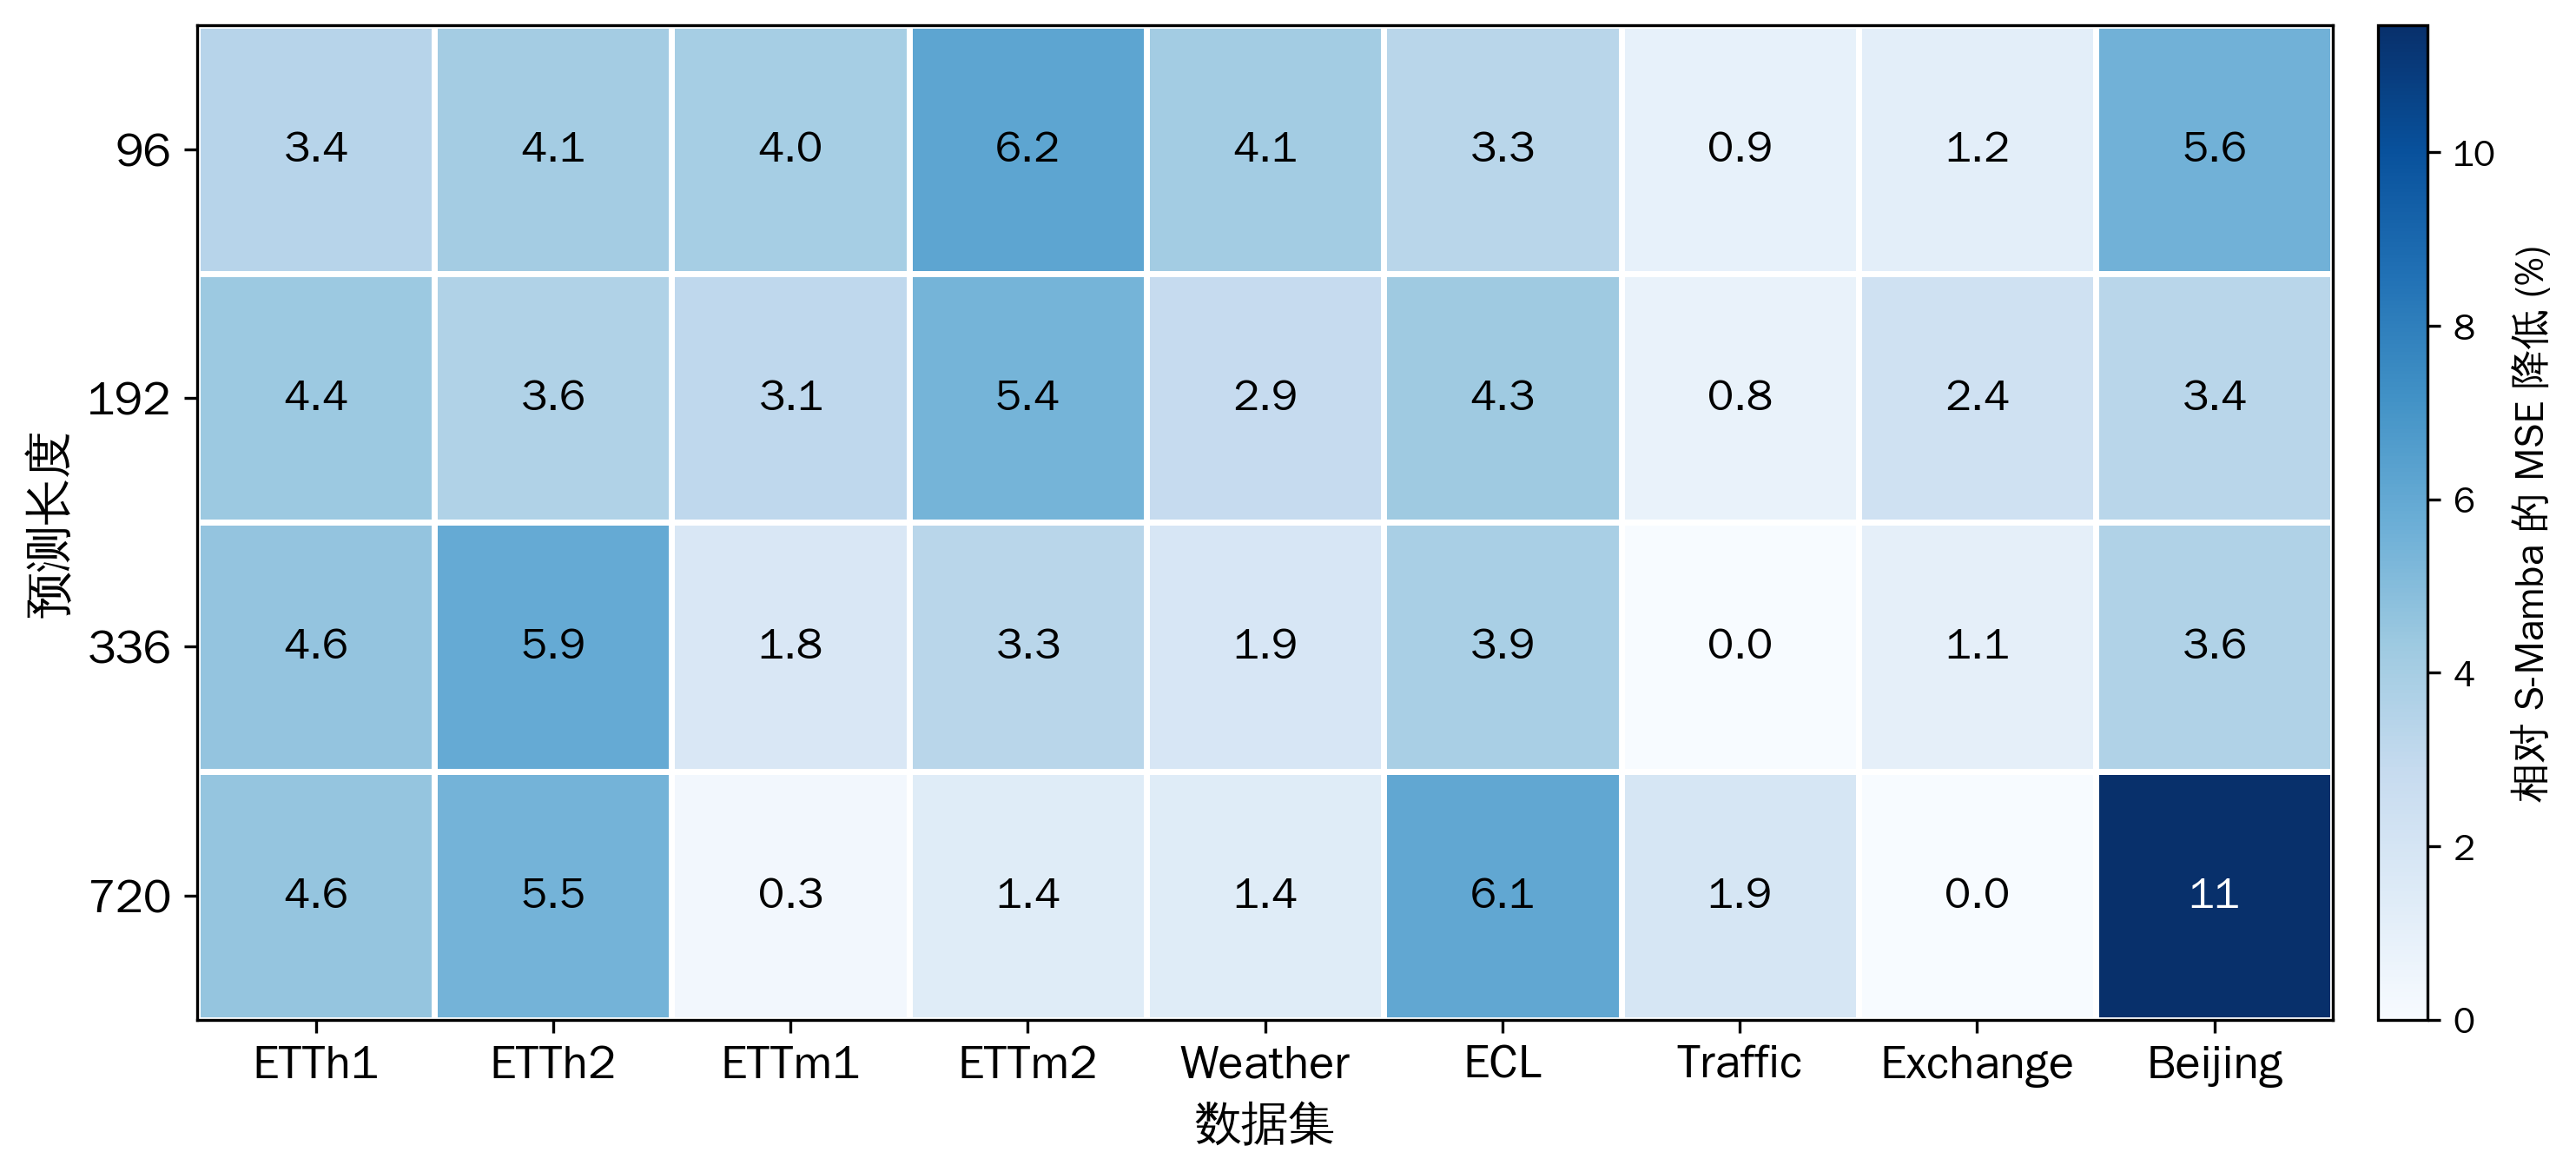
\includegraphics[width=0.938\textwidth]{ch5/figs/ch5_winheat.png}

\end{minipage}

\end{center}

\fi

\subsection{B　消融实验}

消融实验的配置与 A 相同，仅在数据范围与模型变体上不同：消融在 ETTh1、ETTh2、ETTm1、ETTm2 与 Weather 五个数据集上进行，对每个变体分别替换或去掉表 3 所列的组件，主干配置、训练协议与评测口径均与 A 一致。
表 4 在五个数据集上分离量子核与频域监督两组件的贡献。
消融围绕量子核与频域监督两个设计展开，并以同特征维数的 RBF 核作为量子核的经典替代方案。
Full 表示量子核加频域监督的完整模型；
A1 去掉量子核而保留频域监督，用来检验量子核相对主干加频域监督的增量；
A2 把量子核换成同特征维数的 RBF 核而保留频域监督，用来检验量子核相对经典 RBF 核的增量；
A3 保留量子核而去掉频域监督，用来检验频域监督的作用；
A4 在 A2 的基础上去掉频域监督，作为去掉两者的下界参照。
表 3 汇总各变体的组件构成，表 4 给出数值结果。
Full 相对 A2 在多数数据集与预测长度上保持优势，说明性能提升并非仅来自核化操作本身；
频域监督的收益随步长增大。

\begin{center}

\begin{minipage}{\textwidth}

\footnotesize

表 3　各消融变体的组件构成。Full 为 QCCK-M 完整模型；A1 去除量子核，A2 以 RBF 核替代量子核，A3 去除频域监督，A4 同时以 RBF 替代量子核并去除频域监督。\\[2pt]

\centering

\setlength{\tabcolsep}{4pt}

\begin{tabular}{@{}lccc@{}}

\hline

组件 & 量子核 & RBF 核 & 频域监督 \\ \hline

Full & 有 & 无 & 有 \\

A1 & 无 & 无 & 有 \\

A2 & 无 & 有 & 有 \\

A3 & 有 & 无 & 无 \\

A4 & 无 & 有 & 无 \\

\hline

\end{tabular}

\end{minipage}

\end{center}

\begin{center}

\begin{minipage}{\textwidth}

\scriptsize

表 4　消融数值结果，每格给出 MSE 与 MAE；其中 Full 一列的数值与主表里 QCCK-M 对应格完全一致，保证两张表自洽。标注规则与表 2 相同。\\[2pt]

\centering

\setlength{\tabcolsep}{4pt}

\begin{tabular}{@{}llccccc@{}}

\hline

数据集 & H & Full & A1 & A2 & A3 & A4 \\ \hline

ETTh1 & 96 & \shortstack{\colorbox[gray]{0.82}{\textbf{0.3745}}\\\colorbox[gray]{0.92}{0.3971}} & \shortstack{\colorbox[gray]{0.92}{0.3757}\\\colorbox[gray]{0.82}{\textbf{0.3969}}} & \shortstack{0.3760\\0.3973} & \shortstack{0.3878\\0.4083} & \shortstack{0.3892\\0.4083} \\ \hline

ETTh1 & 192 & \shortstack{\colorbox[gray]{0.82}{\textbf{0.4255}}\\\colorbox[gray]{0.82}{\textbf{0.4271}}} & \shortstack{\colorbox[gray]{0.92}{0.4269}\\\colorbox[gray]{0.92}{0.4278}} & \shortstack{\colorbox[gray]{0.92}{0.4269}\\0.4282} & \shortstack{0.4398\\0.4388} & \shortstack{0.4397\\0.4388} \\ \hline

ETTh1 & 336 & \shortstack{\colorbox[gray]{0.82}{\textbf{0.4678}}\\\colorbox[gray]{0.82}{\textbf{0.4489}}} & \shortstack{0.4695\\0.4518} & \shortstack{\colorbox[gray]{0.92}{0.4691}\\\colorbox[gray]{0.92}{0.4515}} & \shortstack{0.4935\\0.4711} & \shortstack{0.4974\\0.4735} \\ \hline

ETTh1 & 720 & \shortstack{\colorbox[gray]{0.82}{\textbf{0.4833}}\\\colorbox[gray]{0.82}{\textbf{0.4849}}} & \shortstack{0.4948\\0.4932} & \shortstack{\colorbox[gray]{0.92}{0.4924}\\\colorbox[gray]{0.92}{0.4907}} & \shortstack{0.5058\\0.4959} & \shortstack{0.5082\\0.4967} \\ \hline

ETTh2 & 96 & \shortstack{\colorbox[gray]{0.82}{\textbf{0.2849}}\\\colorbox[gray]{0.92}{0.3367}} & \shortstack{\colorbox[gray]{0.92}{0.2853}\\\colorbox[gray]{0.82}{\textbf{0.3362}}} & \shortstack{0.2882\\0.3392} & \shortstack{0.2979\\0.3498} & \shortstack{0.2962\\0.3480} \\ \hline

ETTh2 & 192 & \shortstack{\colorbox[gray]{0.82}{\textbf{0.3646}}\\\colorbox[gray]{0.82}{\textbf{0.3886}}} & \shortstack{\colorbox[gray]{0.92}{0.3683}\\\colorbox[gray]{0.92}{0.3888}} & \shortstack{0.3688\\0.3891} & \shortstack{0.3801\\0.4005} & \shortstack{0.3793\\0.3996} \\ \hline

ETTh2 & 336 & \shortstack{\colorbox[gray]{0.82}{\textbf{0.4002}}\\\colorbox[gray]{0.82}{\textbf{0.4170}}} & \shortstack{\colorbox[gray]{0.92}{0.4089}\\\colorbox[gray]{0.92}{0.4209}} & \shortstack{0.4119\\0.4230} & \shortstack{0.4239\\0.4348} & \shortstack{0.4208\\0.4323} \\ \hline

ETTh2 & 720 & \shortstack{\colorbox[gray]{0.82}{\textbf{0.4084}}\\\colorbox[gray]{0.82}{\textbf{0.4333}}} & \shortstack{0.4139\\0.4356} & \shortstack{\colorbox[gray]{0.92}{0.4115}\\\colorbox[gray]{0.92}{0.4354}} & \shortstack{0.4277\\0.4432} & \shortstack{0.4238\\0.4422} \\ \hline

ETTm1 & 96 & \shortstack{\colorbox[gray]{0.82}{\textbf{0.3180}}\\\colorbox[gray]{0.82}{\textbf{0.3554}}} & \shortstack{\colorbox[gray]{0.92}{0.3236}\\\colorbox[gray]{0.92}{0.3569}} & \shortstack{0.3246\\0.3574} & \shortstack{0.3344\\0.3688} & \shortstack{0.3375\\0.3702} \\ \hline

ETTm1 & 192 & \shortstack{\colorbox[gray]{0.82}{\textbf{0.3661}}\\\colorbox[gray]{0.82}{\textbf{0.3808}}} & \shortstack{0.3717\\0.3854} & \shortstack{\colorbox[gray]{0.92}{0.3711}\\\colorbox[gray]{0.92}{0.3846}} & \shortstack{0.3933\\0.4034} & \shortstack{0.3865\\0.3984} \\ \hline

ETTm1 & 336 & \shortstack{\colorbox[gray]{0.82}{\textbf{0.4023}}\\\colorbox[gray]{0.82}{\textbf{0.4068}}} & \shortstack{\colorbox[gray]{0.92}{0.4130}\\\colorbox[gray]{0.92}{0.4133}} & \shortstack{0.4176\\0.4159} & \shortstack{0.4225\\0.4219} & \shortstack{0.4153\\0.4176} \\ \hline

ETTm1 & 720 & \shortstack{\colorbox[gray]{0.82}{\textbf{0.4727}}\\\colorbox[gray]{0.82}{\textbf{0.4493}}} & \shortstack{0.5232\\0.4793} & \shortstack{0.5194\\0.4774} & \shortstack{\colorbox[gray]{0.92}{0.5051}\\\colorbox[gray]{0.92}{0.4644}} & \shortstack{0.5055\\\colorbox[gray]{0.92}{0.4644}} \\ \hline

ETTm2 & 96 & \shortstack{\colorbox[gray]{0.82}{\textbf{0.1704}}\\\colorbox[gray]{0.82}{\textbf{0.2515}}} & \shortstack{\colorbox[gray]{0.92}{0.1734}\\\colorbox[gray]{0.92}{0.2533}} & \shortstack{0.1742\\0.2539} & \shortstack{0.1817\\0.2664} & \shortstack{0.1820\\0.2650} \\ \hline

ETTm2 & 192 & \shortstack{\colorbox[gray]{0.82}{\textbf{0.2387}}\\\colorbox[gray]{0.82}{\textbf{0.2959}}} & \shortstack{0.2441\\0.2997} & \shortstack{\colorbox[gray]{0.92}{0.2438}\\\colorbox[gray]{0.92}{0.2991}} & \shortstack{0.2486\\0.3087} & \shortstack{0.2496\\0.3097} \\ \hline

ETTm2 & 336 & \shortstack{\colorbox[gray]{0.82}{\textbf{0.3022}}\\\colorbox[gray]{0.82}{\textbf{0.3375}}} & \shortstack{\colorbox[gray]{0.92}{0.3059}\\\colorbox[gray]{0.92}{0.3391}} & \shortstack{0.3132\\0.3431} & \shortstack{0.3184\\0.3517} & \shortstack{0.3174\\0.3518} \\ \hline

ETTm2 & 720 & \shortstack{\colorbox[gray]{0.82}{\textbf{0.4077}}\\\colorbox[gray]{0.82}{\textbf{0.3976}}} & \shortstack{0.4201\\0.4044} & \shortstack{\colorbox[gray]{0.92}{0.4107}\\\colorbox[gray]{0.92}{0.4010}} & \shortstack{0.4312\\0.4144} & \shortstack{0.4279\\0.4137} \\ \hline

Weather & 96 & \shortstack{\colorbox[gray]{0.82}{\textbf{0.1581}}\\\colorbox[gray]{0.82}{\textbf{0.1997}}} & \shortstack{0.1598\\\colorbox[gray]{0.92}{0.2015}} & \shortstack{\colorbox[gray]{0.92}{0.1596}\\0.2022} & \shortstack{0.1660\\0.2095} & \shortstack{0.1655\\0.2092} \\ \hline

Weather & 192 & \shortstack{\colorbox[gray]{0.82}{\textbf{0.2092}}\\\colorbox[gray]{0.82}{\textbf{0.2476}}} & \shortstack{0.2108\\0.2486} & \shortstack{\colorbox[gray]{0.92}{0.2106}\\\colorbox[gray]{0.92}{0.2484}} & \shortstack{0.2153\\0.2543} & \shortstack{0.2141\\0.2537} \\ \hline

Weather & 336 & \shortstack{\colorbox[gray]{0.82}{\textbf{0.2680}}\\\colorbox[gray]{0.82}{\textbf{0.2918}}} & \shortstack{\colorbox[gray]{0.92}{0.2693}\\\colorbox[gray]{0.92}{0.2922}} & \shortstack{0.2696\\0.2933} & \shortstack{0.2733\\0.2965} & \shortstack{0.2732\\0.2967} \\ \hline

Weather & 720 & \shortstack{\colorbox[gray]{0.82}{\textbf{0.3483}}\\\colorbox[gray]{0.82}{\textbf{0.3444}}} & \shortstack{0.3511\\0.3473} & \shortstack{\colorbox[gray]{0.92}{0.3506}\\\colorbox[gray]{0.92}{0.3465}} & \shortstack{0.3551\\0.3493} & \shortstack{0.3544\\0.3478} \\ \hline

\end{tabular}

\end{minipage}

\end{center}

\subsection{C　机制验证}

机制验证沿用 A 的模型，不重新训练，仅在评测方式上不同：固定 ETTh1 与 ETTm2 的 96 步设置，取测试集的前八个样本，对输入施加扰动并比较扰动前后的预测。
具体做法是：扰动加在归一化后的输入窗口 $b_x$ 上，位于进入编码器嵌入层之前，也就是初始输入观测值这一层；解码器的标签段与模型内部的任何一层都不改动。
扰动对第 j 个变量整列施加，96 个时间步加的是同一个常数，即扰动量沿时间维广播，而不是逐点噪声。
扰动幅度取 $0.1\sigma_j$，其中 $\sigma_j$ 为该样本内第 j 个变量沿时间维的标准差；注意这里是归一化后数值的标准差，不是原始量纲。
扰动正负号随机，每个变量重复三次以抵消随机性；
记扰动前后的预测为 $\hat{y}$ 与 $\hat{y}'$，则输出通道 i 对输入变量 j 的相对响应定义为 $S[i,j]$ = $\|\hat{y}'_i-\hat{y}_i\|/\|\hat{y}_i\|$，即该通道预测序列的变化幅度相对于自身预测幅度的比例，除以自身范数是为了让不同量级的变量可比。
把 S 的对角元素平均得到对角响应，代表变量对自身的影响；把非对角元素平均得到非对角响应，代表变量对其它变量的影响；两者之比即跨变量影响相对于自身影响的强度。
主干对跨变量输入近乎不敏感。我们在 ETTh1 的 96 步设置上，对每个输入通道施加一个小扰动，测各输出通道的相对响应。
表 5 在两个数据集上给出同一现象。基线主干的非对角响应约为 1e-7，非对角与对角响应之比约为 1e-6，即一个变量的输出几乎不受其它变量输入的影响；
加入耦合模块后，非对角响应上升到约 2e-4 到 4e-4，比值上升到 1e-3 到 1e-2 量级，跨变量响应提升约三个数量级甚至更高。
这是本方法立足点的直接定量证据。

\begin{center}

\begin{minipage}{\textwidth}

\footnotesize

表 5　ETTh1 与 ETTm2 在 96 步上的跨变量输入灵敏度，即非对角与对角响应之比。\\[2pt]

\centering

\setlength{\tabcolsep}{4pt}

\begin{tabular}{@{}lcccc@{}}

\hline

数据集 & 模型 & 非对角响应 & 对角响应 & 比值 \\ \hline

ETTh1 & S-Mamba & 1.1e-7 & 9.6e-2 & 1.2e-6 \\

ETTh1 & QCCK-M & 2.4e-4 & 1.0e-1 & 2.3e-3 \\

ETTm2 & S-Mamba & 7.4e-8 & 4.6e-2 & 1.6e-6 \\

ETTm2 & QCCK-M & 3.6e-4 & 4.8e-2 & 7.5e-3 \\

\hline

\end{tabular}

\end{minipage}

\end{center}

\subsection{D　可解释性}

可解释性建立在原始保真度核 f 之上。
为与第三章的定义保持一致，这里展示 $f[i,j]=|\langle\psi_i|\psi_j\rangle|^2$，它对称、对角为 1、取值在 0 到 1 之间，因此每个元素都能直接读出对应变量对之间的耦合强弱，不需要额外的注意力权重或归因步骤。
把测试样本上的 f 平均后我们看到，在七变量的共址系统 ETTh1 与 ETTm2 上，大多数变量对的耦合都很小，少数强耦合对显著突出：强度超过 0.1 的强对约占全部变量对的 10\%，其中 ETTh1 上最强的一对耦合值约 0.60；
在变量数为 321 的 ECL 与 862 的 Traffic 上，非对角均值更低，强度超过 0.1 的强对占比约 1\%。
图 3a 与图 3b 直接展示这两个七变量系统的非对角耦合，格内数值即对应变量对的耦合强度：最强两对 HUFL–MUFL 与 HULL–MULL 的取值约 0.60 与 0.31，明显高于其余变量对。我们还校验了长预测长度：图 3d 给出 ETTh1 在 720 步下的结构，其最强耦合对约 0.83，且主要强耦合变量对在不同预测长度下保持一致，例如 HUFL-MUFL 与 HULL-MULL，说明模型捕获了具有持续性的变量关系。

\ifchfivefigs

\begin{center}

\begin{minipage}{\textwidth}

\footnotesize

图 3a　ETTh1 在 96 步预测长度下的平均保真度核 f 非对角，轴为真实变量名，格内数值为对应变量对的耦合值；对角元素恒为 1，可视化时隐藏。\\[2pt]

\centering

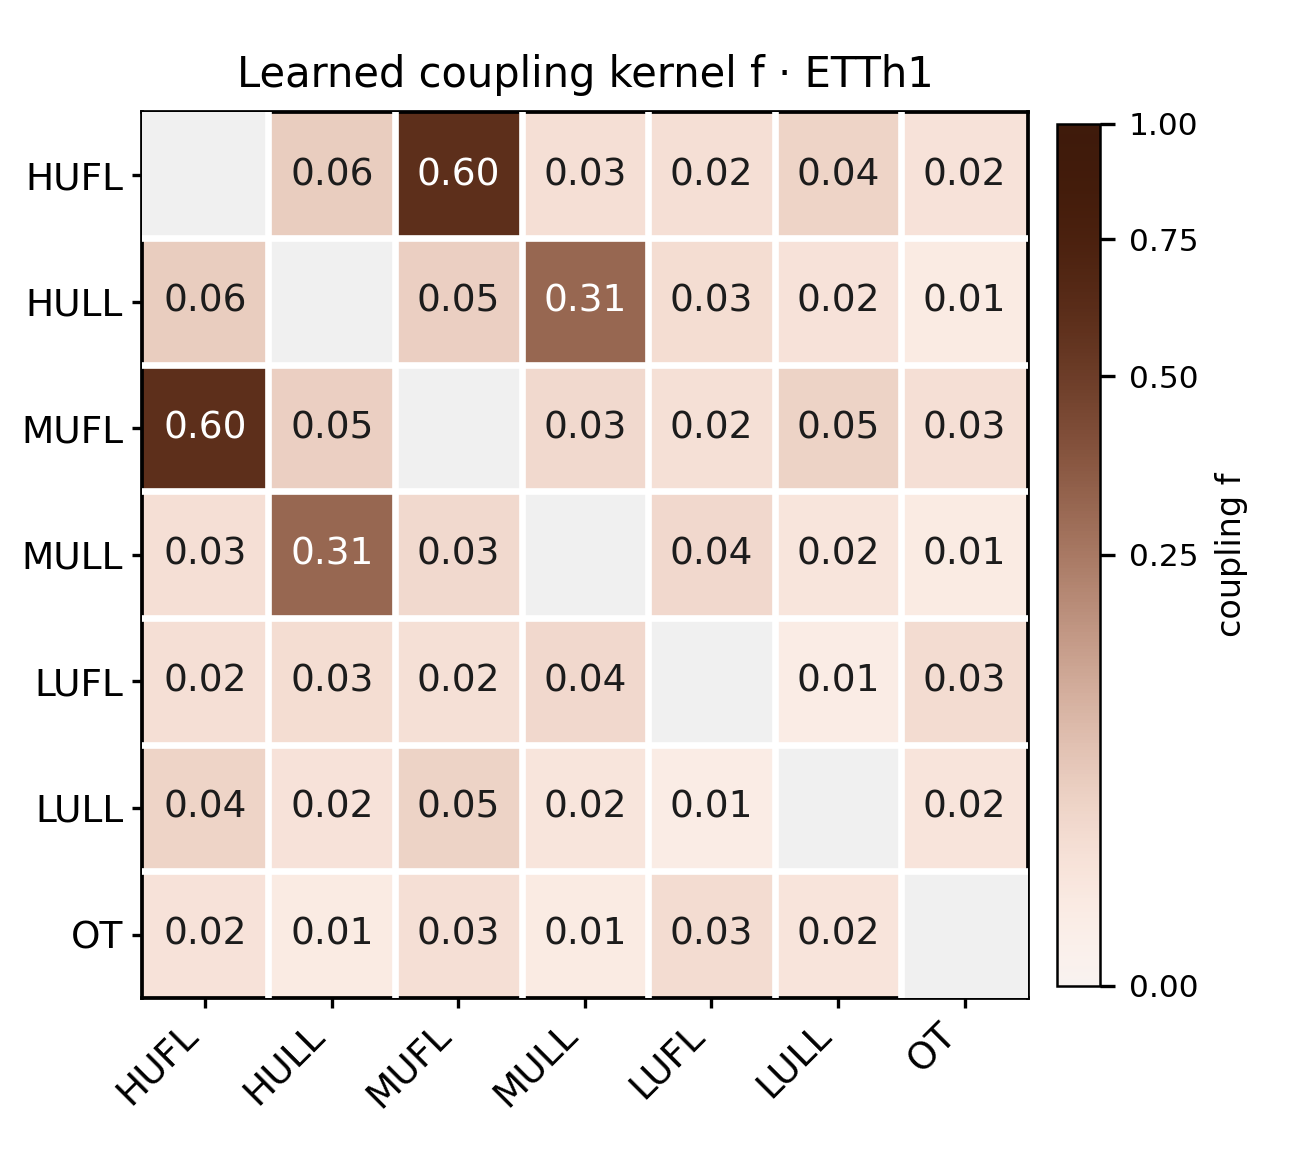
\includegraphics[width=0.475\textwidth]{ch5/figs/ch5_k_ETTh1.png}

\end{minipage}

\end{center}

\fi

\ifchfivefigs

\begin{center}

\begin{minipage}{\textwidth}

\footnotesize

图 3b　ETTm2 在 96 步预测长度下的平均保真度核 f 非对角。\\[2pt]

\centering

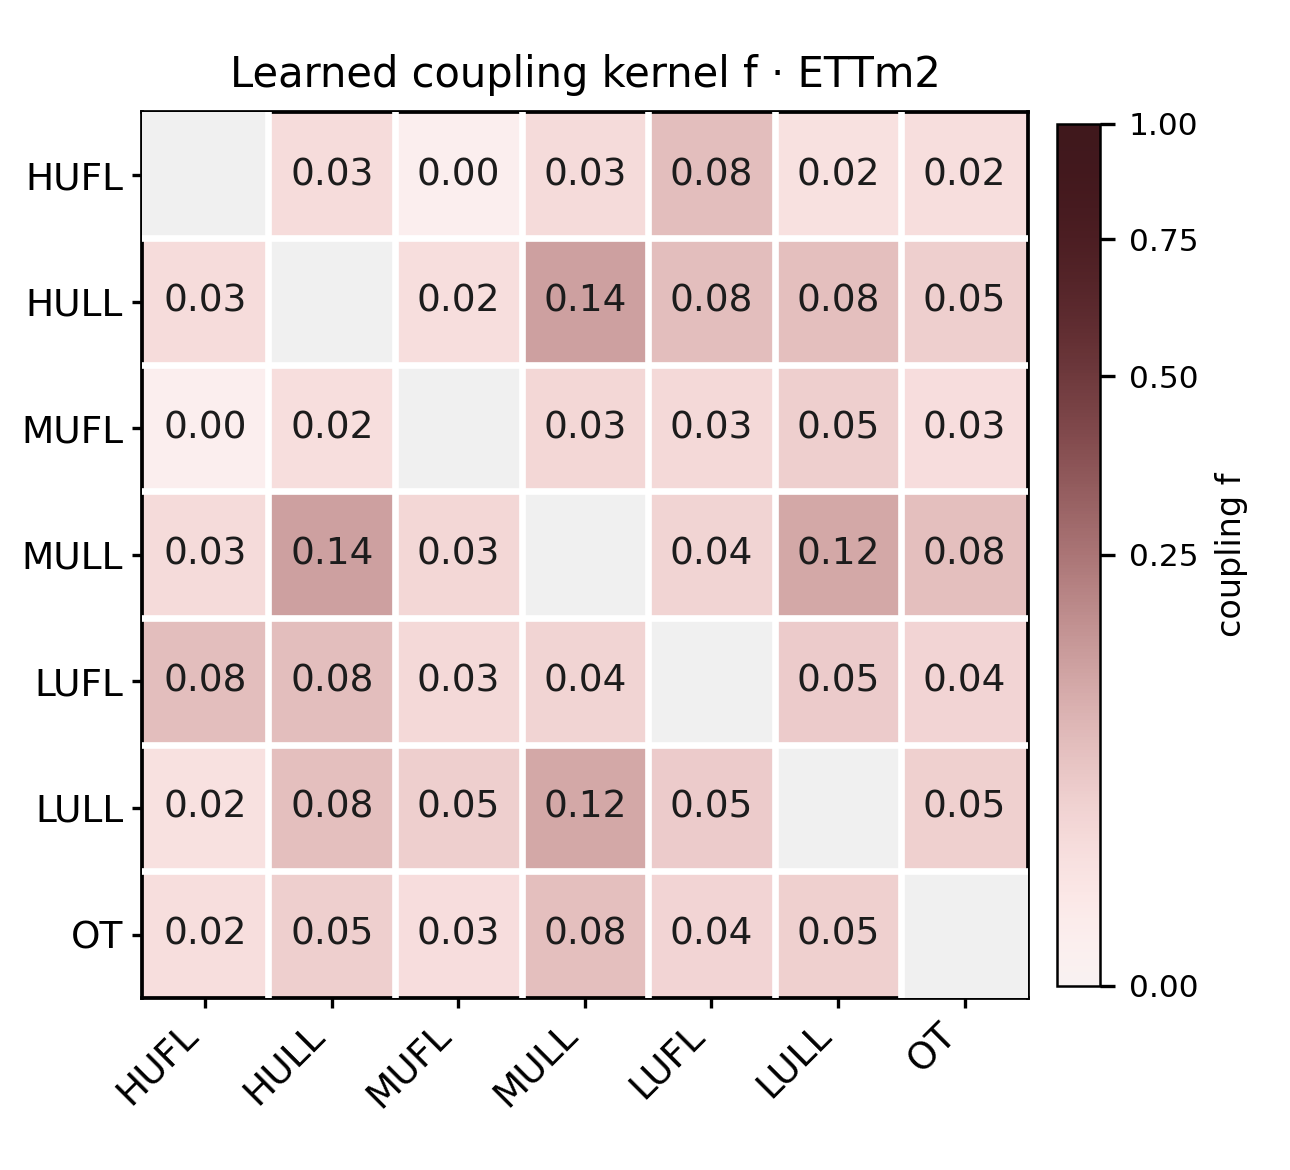
\includegraphics[width=0.475\textwidth]{ch5/figs/ch5_k_ETTm2.png}

\end{minipage}

\end{center}

\fi

ETTh1 的七个通道取自同一变电站：HUFL、HULL、MUFL、MULL、LUFL、LULL 分别是高压、中压、低压三个电压等级下的有用负荷与无用负荷，OT 为变压器油温。模型给出的耦合结构与这一物理分组吻合。
最强的一对是 HUFL 与 MUFL，耦合值 0.60，其次是 HULL 与 MULL，耦合值 0.31：前者是高压与中压的有用负荷，后者是高压与中压的无用负荷，即相邻电压层级上同类负荷之间的耦合最强。
相比之下，同一电压层级内有用负荷与无用负荷之间的耦合很弱，HUFL 与 HULL 只有 0.06，MUFL 与 MULL 只有 0.03，说明模型区分的是负荷的用途，而不是电压层级本身。
低压通道与其余通道普遍耦合很低，LUFL 与 LULL 各自与其余通道的平均耦合都在 0.03 以下，与低压侧负荷独立性强、对整站负荷驱动作用小一致。
油温 OT 与各负荷通道的耦合最弱，与其余通道的平均耦合只有 0.02，其中与 HULL 仅 0.01，这与油温是变压器负载的结果量、而非驱动量相符。
按通道看，与其余通道的平均耦合从高到低依次为高压与中压的有用负荷、高压与中压的无用负荷、低压负荷、油温，这一顺序与各通道在配电系统中的位置一致。

\ifchfivefigs

\begin{center}

\begin{minipage}{\textwidth}

\footnotesize

图 3d　ETTh1 在 720 步预测长度下的平均保真度核 f 非对角，用于比较不同预测长度下主要变量耦合关系。\\[2pt]

\centering

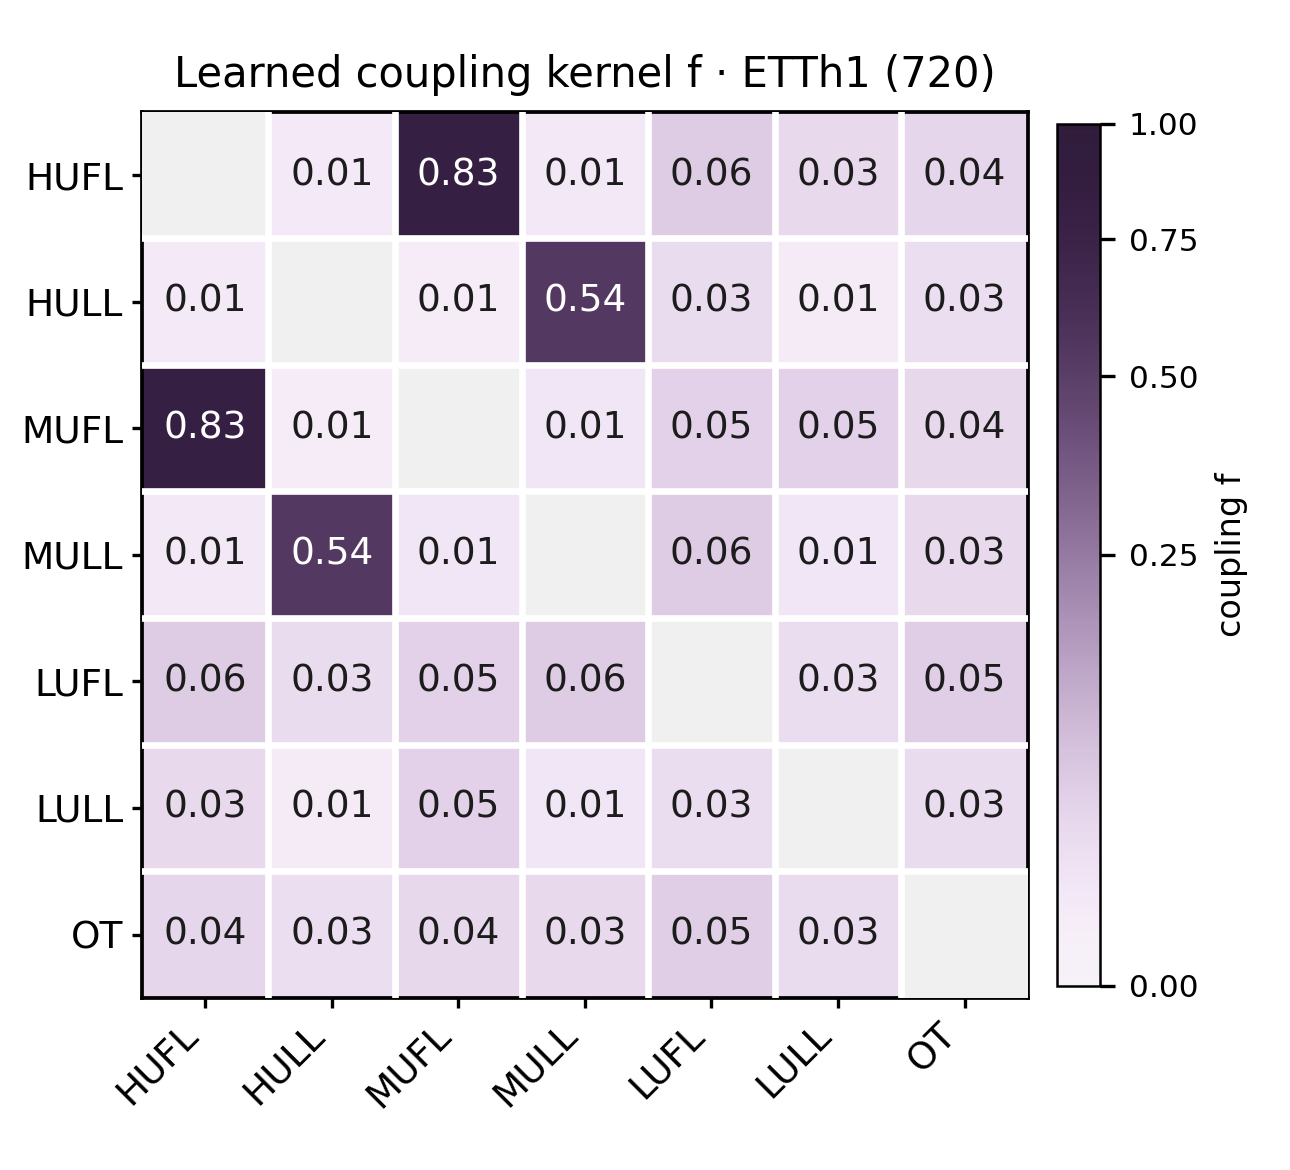
\includegraphics[width=0.475\textwidth]{ch5/figs/ch5_k_ETTh1_720.png}

\end{minipage}

\end{center}

\fi

不同数据集耦合分布的对比。
图 3c 用经验累计分布函数（Empirical Cumulative Distribution Function，ECDF）比较四类数据集非对角耦合值的分布：对每个数据集，我们收集平均 f 的全部非对角元素，纵轴给出不超过横轴对应耦合值的变量对比例。曲线在低值处快速上升，表示该数据集的耦合结构稀疏、绝大多数变量对耦合很弱；曲线整体更靠右，则表示存在更多强耦合对。
这里 ETTh1 与 ETTm2 上超过 0.1 的强对约占 10\%，而 ECL 与 Traffic 只约占 1\%，说明后者绝大多数变量对耦合微弱。该函数只用于描述不同数据集变量关系的稀疏与强弱，不用于声称预测性能。

\ifchfivefigs

\begin{center}

\begin{minipage}{\textwidth}

\footnotesize

图 3c　ETTh1、ETTm2、ECL 与 Traffic 非对角保真度核 f 值的经验累计分布函数（ECDF）：横轴为变量对的耦合强度 f，纵轴为不超过该值的变量对比例。\\[2pt]

\centering

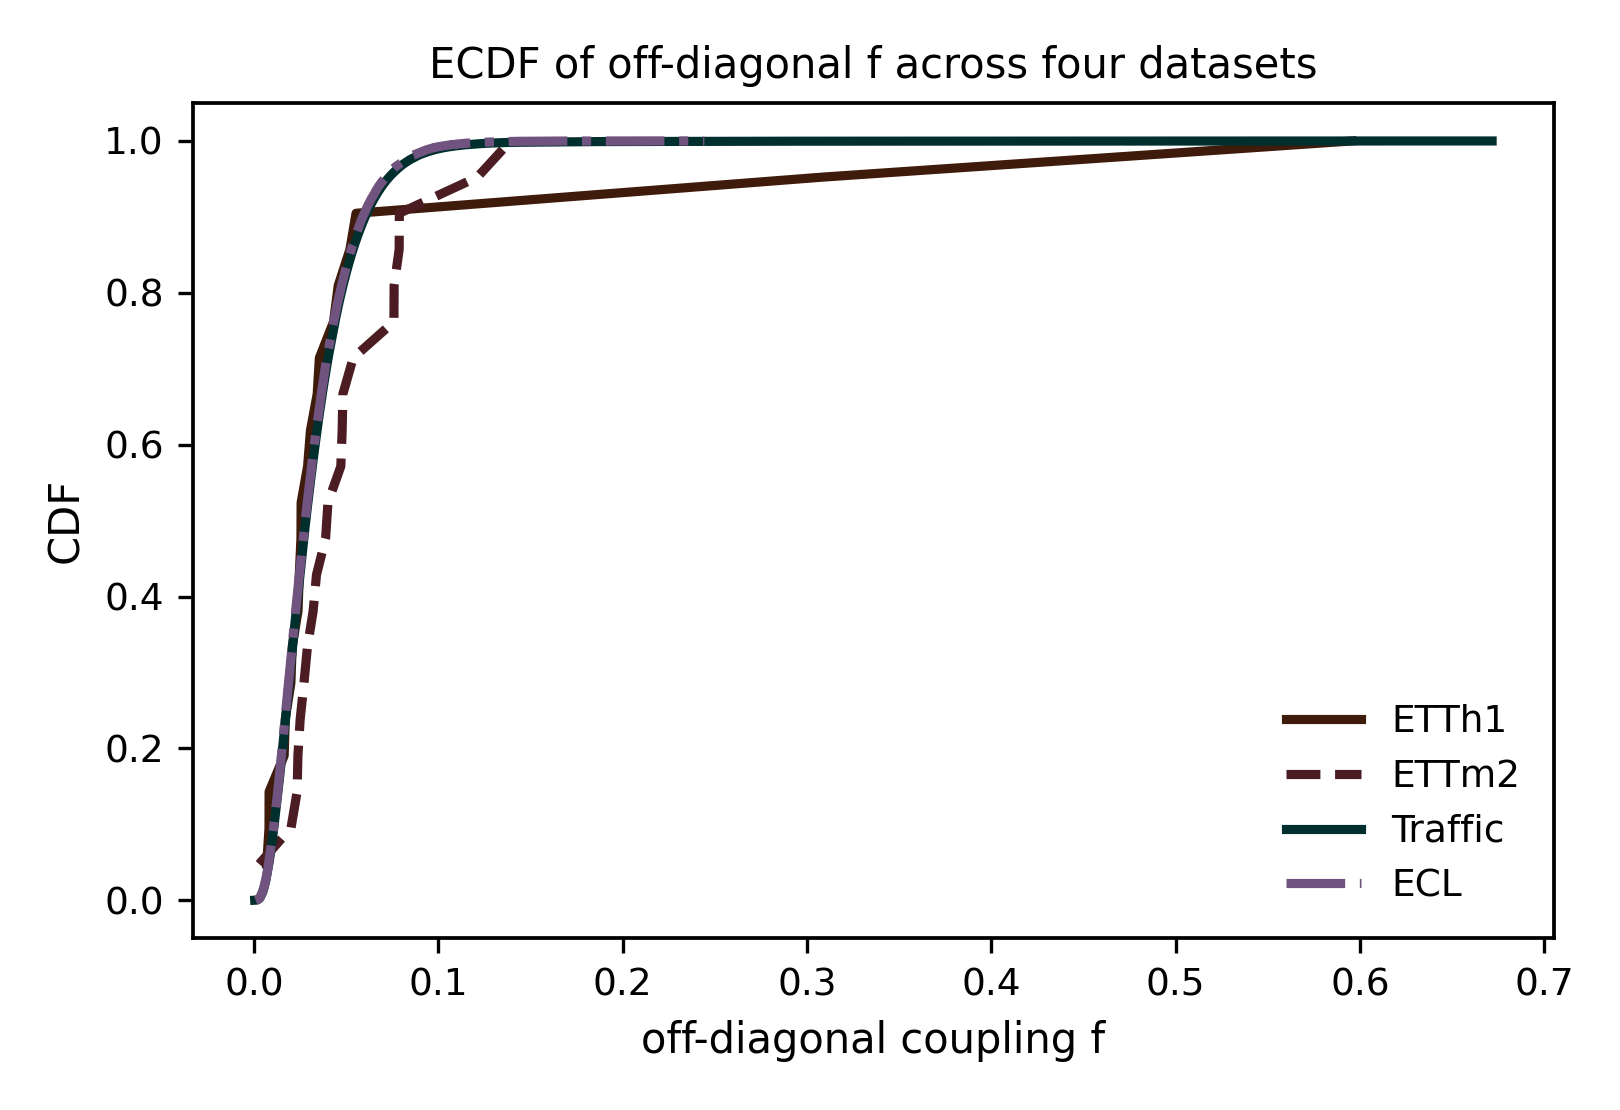
\includegraphics[width=0.656\textwidth]{ch5/figs/ch5_k_dist.png}

\end{minipage}

\end{center}

\fi

图 4 给出一个定性案例。在 ETTh1 的 96 步预测上，油温 OT 的真实曲线、基线主干与 QCCK-M 的预测如图所示：基线主干的预测整体偏低并在上升段明显滞后，QCCK-M 则更好地跟随了真值的走势，前 60 步的 MSE 由 0.0293 降到 0.0143。
这一案例与上文的耦合结构一致，耦合矩阵中读出的通道间强弱关系，在预测中体现为模型对不同通道的跟随能力。

\ifchfivefigs

\begin{center}

\begin{minipage}{\textwidth}

\footnotesize

图 4　ETTh1 在 96 步预测下 OT 通道的定性案例（真值、S-Mamba 与 QCCK-M）。\\[2pt]

\centering

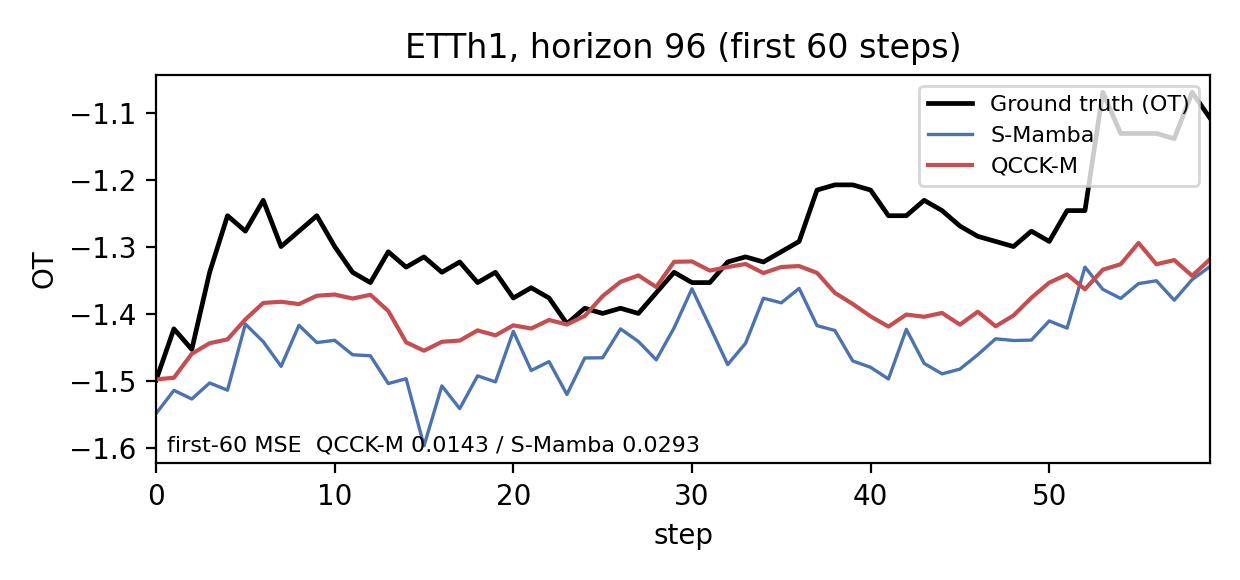
\includegraphics[width=0.812\textwidth]{ch5/figs/ch5_pred_ETTh1.png}

\end{minipage}

\end{center}

\fi

% [已移出] 参考文献块已挪到 references.tex（排在第六章结论之后），由 main.tex 统一 \input。

%% ============================================================
%% 第六章 结论（中文版）
%% 结构：① 提出 QCCK + 作用 → ② QCCK 的内容 → ③ 进一步提出 QCCK-M
%%       → ④ 实验（最好的三个 + 可解释性） → ⑤ 意义与展望（意义写多一点）
%% 纪律：不写预测窗口、不写平均；实验只放 Beijing / ETTm2 / ECL 三个降幅。
%% 编译：xelatex（ctex）
%% ============================================================

\section{结论}

本文提出了量子跨变量耦合核 QCCK，用于在多变量时间序列预测中显式地构造变量之间的耦合关系。
与以扫描或注意力隐式传递变量信息的方式不同，QCCK 把变量间的依赖度量成一份可直接读取的矩阵，使跨变量建模的依据从黑盒权重中分离出来。

QCCK 由频域对齐、量子编码与量子核三个环节构成。
频域对齐在时间轴与频率轴上分别消除变量间的时移与周期尺度差异，把每个变量的原始序列变换为对齐频谱。
量子编码通过振幅通道与相位通道把变量自身特征与频域信息分别加载到量子态的振幅与相位上，得到纠缠量子态。
量子核以两个量子态的重叠程度度量变量间的耦合强度，输出取值在 0 到 1 之间的耦合矩阵 $K$。

在 QCCK 的基础上，本文进一步构建了多变量时间序列预测网络 QCCK-M。
QCCK-M 把 QCCK 以耦合层的形式嵌入主干编码器层之间，使耦合矩阵直接参与跨变量信息融合，在保留主干时序建模能力的同时引入显式的变量间依赖。

实验结果表明，QCCK-M 在多个公开数据集上优于现有方法，其中在 Beijing 数据集上 MSE 降低 11\%，在 ETTm2 上降低 6.2\%，在 ECL 上降低 6.1\%。
此外，耦合矩阵以显式数值呈现变量间的耦合强度，在 ETTh1 等系统上，模型读出的强耦合变量对与数据本身的物理分组一致，说明模型所依据的变量关系可以被直接读取与核对。

随着多变量时间序列应用场景的不断扩展，变量之间的关系往往是决定预测精度的关键，而这类关系通常难以从数据中直接读出。
QCCK 提供了一种把耦合显式化的建模途径，使变量间依赖既能被模型利用，也能被人核对；量子核在其中的作用表明，量子方法不仅可以用于提升表达能力，也可以为模型的可解释性提供支撑。
未来工作将进一步扩展耦合的刻画范围，使 QCCK 能够适应规模更大、耦合形态更复杂的多变量系统，并推动显式耦合建模在更多实际场景中的落地。


\appendix
\renewcommand{\theequation}{A.\arabic{equation}}
\setcounter{equation}{0}
%% ============================================================
%% 附录 A 量子门与量子电路（中文版）
%% 作用：承接第二章 2.1「其具体定义见附录 A」的指向。
%% 内容：量子比特与量子态记号 → 量子门定义 → 本文用到的
%%       单比特旋转门 RY / RZ → 双比特纠缠门 CNOT → 参数化量子线路。
%% 纪律：只作定义性陈述，给出符号含义与作用，不评价意义。
%% 编译：xelatex（ctex）；由 main.tex 以 \appendix 引入，编号为 A。
%% ============================================================

\section{量子门与量子电路}\label{app:quantum}

本附录给出 2.1 节所述量子门与量子电路的具体定义，包括量子比特与量子态的记号、量子门的定义、本文所用到的单比特旋转门 $R_Y$ 与 $R_Z$、双比特纠缠门 CNOT，以及由这些门构成的参数化量子线路。

\subsection{量子比特与量子态}

量子比特是量子计算的基本信息单元，其状态记作 $|\psi\rangle = \alpha|0\rangle + \beta|1\rangle$，其定义如式~(\ref{eq:app-qubit}) 所示。
\begin{equation}
\label{eq:app-qubit}
|\psi\rangle = \alpha\,|0\rangle + \beta\,|1\rangle,\qquad |\alpha|^2+|\beta|^2=1,
\end{equation}
式中 $|0\rangle$、$|1\rangle$ 为一组标准正交基，称为计算基；$\alpha,\beta\in\mathbb{C}$ 为振幅，其模方 $|\alpha|^2$、$|\beta|^2$ 分别给出测量后得到 $|0\rangle$、$|1\rangle$ 的概率。

$n$ 个量子比特构成一个系统，其状态位于 $2^n$ 维复希尔伯特空间 $\mathbb{C}^{2^n}$ 之中，计算基记作 $|b\rangle$，其中 $b\in\{0,1\}^n$ 为比特串，共有 $2^n$ 个，系统的状态为各计算基的叠加，其定义如式~(\ref{eq:app-nqubit}) 所示。
\begin{equation}
\label{eq:app-nqubit}
|\psi\rangle = \sum_{b\in\{0,1\}^n} a_b\,|b\rangle,\qquad \sum_{b\in\{0,1\}^n}|a_b|^2 = 1,
\end{equation}
式中 $a_b$ 为计算基 $|b\rangle$ 的振幅。把 $|\psi\rangle$ 与 $|\phi\rangle$ 两个子系统的状态组合为整体状态时使用张量积 $|\psi\rangle\otimes|\phi\rangle$，该式常简记为 $|\psi\rangle|\phi\rangle$。

\subsection{量子门}

量子门是作用在量子比特状态上的酉算符，其定义如式~(\ref{eq:app-gate}) 所示。
\begin{equation}
\label{eq:app-gate}
|\psi\rangle \mapsto U\,|\psi\rangle,\qquad U^{\dagger}U = I,
\end{equation}
式中 $U$ 为量子门的算符形式，$U^{\dagger}$ 为其共轭转置，$I$ 为单位阵。酉性保证变换后各振幅的模方之和仍为 1，因此量子门的演化不改变测量概率的归一化。

在计算基下，作用于 $n$ 个量子比特的门表示为 $2^n\times 2^n$ 的酉矩阵，其中只作用于单个量子比特的门称为单比特门，其形式为 $2\times 2$ 的酉矩阵。
量子门分为两类：单比特门只改变该比特自身的振幅与相位；同时作用于多个量子比特的门能够在比特之间建立关联，这类门称为纠缠门。
把若干量子门按时间顺序依次施加到量子比特上，即多个酉算符依序相乘，得到的整体算符 $U = U_1 U_2 \cdots U_k$ 就构成量子电路的一次演化。

\subsection{单比特旋转门}

参数化旋转门以旋转角为参数，使量子比特的状态绕指定的坐标轴连续旋转。绕 $Y$ 轴的旋转门 $R_Y$ 的定义如式~(\ref{eq:app-ry}) 所示。
\begin{equation}
\label{eq:app-ry}
R_Y(\theta) = \cos\frac{\theta}{2}\,I - i\sin\frac{\theta}{2}\,Y = \begin{pmatrix} \cos\frac{\theta}{2} & -\sin\frac{\theta}{2} \\[3pt] \sin\frac{\theta}{2} & \cos\frac{\theta}{2} \end{pmatrix},
\end{equation}
式中 $\theta$ 为旋转角，$Y=\begin{pmatrix}0&-i\\ i&0\end{pmatrix}$ 为泡利 $Y$ 矩阵。$R_Y$ 改变两个计算基的振幅分配，因而改变测量得到 $|0\rangle$ 与 $|1\rangle$ 的概率。

绕 $Z$ 轴的旋转门 $R_Z$ 的定义如式~(\ref{eq:app-rz}) 所示。
\begin{equation}
\label{eq:app-rz}
R_Z(\theta) = \cos\frac{\theta}{2}\,I - i\sin\frac{\theta}{2}\,Z = \begin{pmatrix} e^{-i\theta/2} & 0 \\ 0 & e^{i\theta/2} \end{pmatrix},
\end{equation}
式中 $Z=\begin{pmatrix}1&0\\0&-1\end{pmatrix}$ 为泡利 $Z$ 矩阵。$R_Z$ 只改变两个计算基之间的相对相位，不改变二者的测量概率。式~(\ref{eq:app-ry}) 与式~(\ref{eq:app-rz}) 中的旋转角 $\theta$ 可取任意实数，选择不同的旋转角即可连续调节该比特的状态。

\subsection{双比特纠缠门}

受控非门 CNOT 是作用在两个量子比特上的纠缠门，其定义如式~(\ref{eq:app-cnot}) 所示。
\begin{equation}
\label{eq:app-cnot}
\mathrm{CNOT} = |0\rangle\langle 0|\otimes I + |1\rangle\langle 1|\otimes X,\qquad X=\begin{pmatrix}0&1\\1&0\end{pmatrix},
\end{equation}
式中 $X$ 为泡利 $X$ 矩阵，$\otimes$ 为张量积。在计算基下，CNOT 按 $|a,b\rangle\mapsto|a,\,a\oplus b\rangle$ 作用，其中第一个比特为控制比特、第二个比特为受控比特，$\oplus$ 为模 2 加法：控制比特为 $|0\rangle$ 时受控比特保持不变，控制比特为 $|1\rangle$ 时受控比特取反。

一个纠缠门作用之后，多个量子比特的整体状态一般不能写成各单比特状态张量积的形式；当系统处于这样的状态时，称这些量子比特之间存在纠缠，此时对其中一个比特的测量结果与其余比特的测量结果相关联。纠缠门的作用是把各比特的振幅与相位耦合起来，其输出能够携带比特之间的关联。

\subsection{参数化量子线路}

参数化量子线路是由单比特旋转门与双比特纠缠门交替构成、且旋转角可学习的一类量子电路。旋转门负责调节各比特的振幅与相位，为线路提供可调节的自由度；纠缠门负责在比特之间建立纠缠，使线路输出能够携带比特之间的关联；旋转角在训练中与其他网络参数一同优化。

本文在 QCCE 中使用的参数化量子线路，由式~(\ref{eq:app-ry})、(\ref{eq:app-rz}) 的旋转门与式~(\ref{eq:app-cnot}) 的纠缠门构成，其对每个变量独立可学习，具体形式如第三章式~(\ref{eq:circuit}) 所示。


%% ============================================================
%% 参考文献（独立文件，排在结论之后）
%% 来源：原挂在 chapter5_qcckm_exp_zh.tex 末尾，因结论一节要排在第五章之后而移出。
%% 排序：按正文首次出现顺序编号（第一章 P1 起）。
%% 口径（2026-09-22 定）：一律引正式发表版本（会议/期刊、卷期页），
%%       确有正式出处者不再挂 arXiv；仅尚无正式出处的预印本保留 arXiv 编号。
%% 编译：xelatex（ctex）
%% ============================================================

\section*{参考文献}

\begin{thebibliography}{17}

\bibitem{liu2024itransformer} Y.~Liu 等. iTransformer: Inverted Transformers Are Effective for Time Series Forecasting. ICLR 2024.

\bibitem{chittoor2025qultsf} H.~H.~S.~Chittoor, P.~R.~Griffin, A.~Neufeld, J.~Thompson, M.~Gu. QuLTSF: Long-Term Time Series Forecasting with Quantum Machine Learning. ICAART 2025, pp.~824--829.

\bibitem{gu2024mamba} A.~Gu, T.~Dao. Mamba: Linear-Time Sequence Modeling with Selective State Spaces. COLM 2024.

\bibitem{wang2025smamba} Z.~Wang, F.~Kong, S.~Feng, M.~Wang, X.~Yang, H.~Zhao, D.~Wang, Y.~Zhang. Is Mamba Effective for Time Series Forecasting? Neurocomputing, vol.~619, art.~129178, 2025.

\bibitem{ma2025timepro} X.~Ma, Z.~Ni, S.~Xiao, X.~Chen. TimePro: Efficient Multivariate Long-term Time Series Forecasting with Variable- and Time-Aware Hyper-state. ICML 2025.

\bibitem{karadag2026msmamba} Y.~M.~Karadag, I.~Talaz, I.~G.~Dino, S.~Kalkan. ms-Mamba: Multi-scale Mamba for Time-Series Forecasting. Neurocomputing, vol.~680, art.~133226, 2026.

\bibitem{jura2025qssm} S.-A.~Jura, M.~Udrescu, A.~Top\^{i}rceanu. Quantum-Optimized Selective State Space Model for Efficient Time Series Prediction. IEEE BigData 2025, pp.~995--1004.

\bibitem{zhao2024qksan} R.-X.~Zhao, J.~Shi, X.~Li. QKSAN: A Quantum Kernel Self-Attention Network. IEEE Trans. Pattern Anal. Mach. Intell., vol.~46, no.~12, pp.~10184--10195, 2024.

\bibitem{bai2024haqjsk} L.~Bai, L.~Cui, Y.~Wang, M.~Li, J.~Li, P.~S.~Yu, E.~R.~Hancock. HAQJSK: Hierarchical-Aligned Quantum Jensen-Shannon Kernels for Graph Classification. IEEE Trans. Knowl. Data Eng., 2024.

\bibitem{bracewell2000fourier} R.~N.~Bracewell. \emph{The Fourier Transform and Its Applications}, 3rd ed. New York, NY, USA: McGraw-Hill, 2000.

\bibitem{zeng2023dlinear} A.~Zeng 等. Are Transformers Effective for Time Series Forecasting. AAAI 2023.

\bibitem{nie2023patchtst} Y.~Nie 等. A Time Series is Worth 64 Words. ICLR 2023.

\bibitem{wu2023timesnet} H.~Wu 等. TimesNet: Temporal 2D-Variation Modeling for General Time Series Analysis. ICLR 2023.

\bibitem{an2026dema} R.~An, H.~Qu, W.~Fan, X.~Shang, Q.~Li. DeMa: Dual-Path Delay-Aware Mamba for Efficient Multivariate Time Series Analysis. arXiv:2601.05527, 2026.

\bibitem{wang2025fredf} H.~Wang, L.~Pan, Y.~Shen, Z.~Chen, D.~Yang, Y.~Yang, S.~Zhang, X.~Liu, H.~Li, D.~Tao. FreDF: Learning to Forecast in the Frequency Domain. ICLR 2025.

\bibitem{zhou2021informer} H.~Zhou 等. Informer: Beyond Efficient Transformer for Long Sequence Time-Series Forecasting. AAAI 2021.

\bibitem{wu2021autoformer} H.~Wu 等. Autoformer: Decomposition Transformers with Auto-Correlation for Long-term Series Forecasting. NeurIPS 2021.

\end{thebibliography}


\end{document}
